% UCL Thesis LaTeX Template
%  (c) Ian Kirker, 2014
% 
% This is a template/skeleton for PhD/MPhil/MRes theses.
%
% It uses a rather split-up file structure because this tends to
%  work well for large, complex documents.
% We suggest using one file per chapter, but you may wish to use more
%  or fewer separate files than that.
% We've also separated out various bits of configuration into their
%  own files, to keep everything neat.
% Note that the \input command just streams in whatever file you give
%  it, while the \include command adds a page break, and does some
%  extra organisation to make compilation faster. Note that you can't
%  use \include inside an \include-d file.
% We suggest using \input for settings and configuration files that
%  you always want to use, and \include for each section of content.
% If you do that, it also means you can use the \includeonly statement
%  to only compile up the section you're currently interested in.
% You might also want to put figures into their own files to be \input.

% For more information on \input and \include, see:
%  http://tex.stackexchange.com/questions/246/when-should-i-use-input-vs-include


% Formatting and binding rules for theses are here: 
%  https://www.ucl.ac.uk/students/exams-and-assessments/research-assessments/format-bind-and-submit-your-thesis-general-guidance

% This package goes first and foremost, because it checks all 
%  your syntax for mistakes and some old-fashioned LaTeX commands.
% Note that normally you should load your documentclass before 
%  packages, because some packages change behaviour based on
%  your document settings.
% Also, for those confused by the RequirePackage here vs usepackage
%  elsewhere, usepackage cannot be used before the documentclass
%  command, while RequirePackage can. That's the only functional
%  difference as far as I'm aware.
\RequirePackage[l2tabu, orthodox]{nag}


% ------ Main document class specification ------
% The draft option here prevents images being inserted,
%  and adds chunky black bars to boxes that are exceeding 
%  the page width (to show that they are).
% The oneside option can optionally be replaced by twoside if
%  you intend to print double-sided. Note that this is
%  *specifically permitted* by the UCL thesis formatting
%  guidelines.
%
% Valid options in terms of type are:
%  phd
%  mres
%  mphil
%\documentclass[12pt,phd,draft,a4paper,oneside]{ucl_thesis}
\documentclass[12pt,phd,a4paper,oneside]{ucl_thesis}


% Package configuration:
%  LaTeX uses "packages" to add extra commands and features.
%  There are quite a few useful ones, so we've put them in a 
%   separate file.
% -------- Packages --------

% This package just gives you a quick way to dump in some sample text.
% You can remove it -- it's just here for the examples.
\usepackage{blindtext}

% This package means empty pages (pages with no text) won't get stuff
%  like chapter names at the top of the page. It's mostly cosmetic.
\usepackage{emptypage}

% The graphicx package adds the \includegraphics command,
%  which is your basic command for adding a picture.
\usepackage{graphicx}

% The float package improves LaTeX's handling of floats,
%  and also adds the option to *force* LaTeX to put the float
%  HERE, with the [H] option to the float environment.
\usepackage{float}

% The amsmath package enhances the various ways of including
%  maths, including adding the align environment for aligned
%  equations.
\usepackage{amsmath}

% Use these two packages together -- they define symbols
%  for e.g. units that you can use in both text and math mode.
\usepackage{gensymb}
\usepackage{textcomp}
% You may also want the units package for making little
%  fractions for unit specifications.
%\usepackage{units}


%%%
\usepackage{mathrsfs} % additional use for different fonts
%\usepackage{hyperref} % additional use hyperref
\usepackage{amsthm} % additional environment
\usepackage{amsmath,amssymb}
\usepackage{caption} % additional picture environment
\usepackage{subcaption} % additional picture environment



% The setspace package lets you use 1.5-sized or double line spacing.
\usepackage{setspace}
\setstretch{1.5}

% That just does body text -- if you want to expand *everything*,
%  including footnotes and tables, use this instead:
%\renewcommand{\baselinestretch}{1.5}


% PGFPlots is either a really clunky or really good way to add graphs
%  into your document, depending on your point of view.
% There's waaaaay too much information on using this to cover here,
%  so, you might want to start here:
%   http://pgfplots.sourceforge.net/
%  or here:
%   http://pgfplots.sourceforge.net/pgfplots.pdf
%\usepackage{pgfplots}
%\pgfplotsset{compat=1.3} % <- this fixed axis labels in the version I was using

% PGFPlotsTable can help you make tables a little more easily than
%  usual in LaTeX.
% If you're going to have to paste data in a lot, I'd suggest using it.
%  You might want to start with the manual, here:
%  http://pgfplots.sourceforge.net/pgfplotstable.pdf
%\usepackage{pgfplotstable}

% These settings are also recommended for using with pgfplotstable.
%\pgfplotstableset{
%	% these columns/<colname>/.style={<options>} things define a style
%	% which applies to <colname> only.
%	empty cells with={--}, % replace empty cells with '--'
%	every head row/.style={before row=\toprule,after row=\midrule},
%	every last row/.style={after row=\bottomrule}
%}


% The mhchem package provides chemistry formula typesetting commands
%  e.g. \ce{H2O}
%\usepackage[version=3]{mhchem}

% And the chemfig package gives a weird command for adding Lewis 
%  diagrams, for e.g. organic molecules
%\usepackage{chemfig}

% The linenumbers command from the lineno package adds line numbers
%  alongside your text that can be useful for discussing edits 
%  in drafts.
% Remove or comment out the command for proper versions.
%\usepackage[modulo]{lineno}
% \linenumbers 


% Alternatively, you can use the ifdraft package to let you add
%  commands that will only be used in draft versions
%\usepackage{ifdraft}

% For example, the following adds a watermark if the draft mode is on.
%\ifdraft{
%  \usepackage{draftwatermark}
%  \SetWatermarkText{\shortstack{\textsc{Draft Mode}\\ \strut \\ \strut \\ \strut}}
%  \SetWatermarkScale{0.5}
%  \SetWatermarkAngle{90}
%}


% The multirow package adds the option to make cells span 
%  rows in tables.
\usepackage{multirow}


% Subfig allows you to create figures within figures, to, for example,
%  make a single figure with 4 individually labeled and referenceable
%  sub-figures.
% It's quite fiddly to use, so check the documentation.
%\usepackage{subfig}

% The natbib package allows book-type citations commonly used in
%  longer works, and less commonly in science articles (IME).
% e.g. (Saucer et al., 1993) rather than [1]
% More details are here: http://merkel.zoneo.net/Latex/natbib.php
%\usepackage{natbib}

% The bibentry package (along with the \nobibliography* command)
%  allows putting full reference lines inline.
%  See: 
%   http://tex.stackexchange.com/questions/2905/how-can-i-list-references-from-bibtex-file-in-line-with-commentary
\usepackage{bibentry} 

% The isorot package allows you to put things sideways 
%  (or indeed, at any angle) on a page.
% This can be useful for wide graphs or other figures.
%\usepackage{isorot}

% The caption package adds more options for caption formatting.
% This set-up makes hanging labels, makes the caption text smaller
%  than the body text, and makes the label bold.
% Highly recommended.
\usepackage[format=hang,font=small,labelfont=bf]{caption}

% If you're getting into defining your own commands, you might want
%  to check out the etoolbox package -- it defines a few commands
%  that can make it easier to make commands robust.
\usepackage{etoolbox}

% The microtype package adds `micro-typographic extensions' which
% generally makes text more readable and hyphenation less likely.
\usepackage{microtype}


% Sets up links within your document, for e.g. contents page entries
%  and references, and also PDF metadata.
% You should edit this!
%%
%% This file uses the hyperref package to make your thesis have metadata embedded in the PDF, 
%%  and also adds links to be able to click on references and contents page entries to go to 
%%  the pages.
%%

% Some hacks are necessary to make bibentry and hyperref play nicely.
% See: http://tex.stackexchange.com/questions/65348/clash-between-bibentry-and-hyperref-with-bibstyle-elsart-harv
\usepackage{bibentry}
\makeatletter\let\saved@bibitem\@bibitem\makeatother
\usepackage[pdftex,hidelinks]{hyperref}
\makeatletter\let\@bibitem\saved@bibitem\makeatother
\makeatletter
\AtBeginDocument{
    \hypersetup{
        pdfsubject={Thesis Subject},
        pdfkeywords={Thesis Keywords},
        pdfauthor={Author},
        pdftitle={Title},
    }
}
\makeatother
    


% And then some settings in separate files.
% These settings are partly from:
%  http://mintaka.sdsu.edu/GF/bibliog/latex/floats.html

% They give LaTeX more options on where to put your figures, and may
%  mean that fewer of your figures end up at the tops of pages far
%  away from the thing they're related to.

% Alters some LaTeX defaults for better treatment of figures:
% See p.105 of "TeX Unbound" for suggested values.
% See pp. 199-200 of Lamport's "LaTeX" book for details.

%   General parameters, for ALL pages:
\renewcommand{\topfraction}{0.9}	% max fraction of floats at top
\renewcommand{\bottomfraction}{0.8}	% max fraction of floats at bottom

%   Parameters for TEXT pages (not float pages):
\setcounter{topnumber}{2}
\setcounter{bottomnumber}{2}
\setcounter{totalnumber}{4}     % 2 may work better
\setcounter{dbltopnumber}{2}    % for 2-column pages
\renewcommand{\dbltopfraction}{0.9}	% fit big float above 2-col. text
\renewcommand{\textfraction}{0.2}	% page must be at least 20% text, 
%                                  less than that and we get a floatpage

%   Parameters for FLOAT pages (not text pages):
\renewcommand{\floatpagefraction}{0.7}	% require fuller float pages
% N.B.: floatpagefraction MUST be less than topfraction !!
\renewcommand{\dblfloatpagefraction}{0.7}	% require fuller float pages

% remember to use [htp] or [htpb] for placement,
% e.g. 
%  \begin{figure}[htp]
%   ...
%  \end{figure}
 % For things like figures and tables
\bibliographystyle{unsrt}   % For bibliographies

% These control how many number sections your subsections will take
%    e.g. Section 2.3.1.5.6.3
%  and how many of those will get put into the contents pages.
\setcounter{secnumdepth}{3}
\setcounter{tocdepth}{3}


\begin{document}

%%%\nobibliography*
% ^-- This is a dumb trick that works with the bibentry package to let
%  you put bibliography entries whereever you like.
% I used this to put references to papers a chapter's work was 
%  published in at the end of that chapter.
% For more information, see: http://stefaanlippens.net/bibentry

% If you haven't finished making your full BibTex file yet, you
%  might find this useful -- it'll just replace all your
%  citations with little superscript notes.
% Uncomment to use.
%\renewcommand{\cite}[1]{\emph{\textsuperscript{[#1]}}}

% At last, content! Remember filenames are case-sensitive and 
%  *must not* include spaces.
% I may change the way this is done in a future version, 
%  but given that some people needed it, if you need a different degree title 
%  (e.g. Master of Science, Master in Science, Master of Arts, etc)
%  uncomment the following 3 lines and set as appropriate (this *has* to be before \maketitle)
% \makeatletter
% \renewcommand {\@degree@string} {Master of Things}
% \makeatother

\title{Understanding the Spatial Association Between Risk Factors and the Prevalence of Diabetes Mellitus in England}
\author{Sheng Hu}
\department{Department of Something}
\maketitle

\begin{abstract} % 300 word limit
Diabetes Mellitus (DM) is a globally prevalent noncommunicable disease, with its prevalence and incidence rising steadily in recent years. While existing research has uncovered a range of risk factors for DM, the vast majority focus on individual-level factors, overlooking the influence of spatial dimensions on DM prevalence. This study aims to explore the spatial distribution patterns of DM prevalence across England at the MSOA level using spatial regression analysis, identifying significant risk factors. The results indicate that there is significant spatial autocorrelation in the prevalence of DM in England, with the social deprivation (IMD decile), Asian population, obesity, and advancing age identified as significant contributing factors, particularly with the social deprivation and Asian population exhibiting spatial spillover effects. Additionally, although obesity prevalence was significant in the OLS model, they did not show spatial effects in the Spatial Durbin Model. By revealing the spatial patterns of diabetes, this study provides new perspectives for public health policy development in England, highlighting the need for comprehensive interventions targeting specific areas and their neighboring locations. Future research could expand spatial analysis's scale and temporal dimensions to understand better the complex interactions and the causality between DM and its risk factors.
\end{abstract}


\declaration


\begin{acknowledgements}
I greatly appreciate my supervisor, Dr. Jens Kandt, for his guidance and support over the past few months.\\

I acknowledge the use of ChatGPT 4 (Open AI, \url{https://chat.openai.com}) to proofread my final draft.
\end{acknowledgements}

\setcounter{tocdepth}{2} 
% Setting this higher means you get contents entries for
%  more minor section headers.

\tableofcontents
\listoffigures
\addcontentsline{toc}{chapter}{List of Figures}
\listoftables
\addcontentsline{toc}{chapter}{List of Tables}





\begin{Acronyms}
\addcontentsline{toc}{chapter}{List of Acronyms}
\begin{tabbing}
\hspace{3cm} \= \kill
AIC \> Akaike Information Criterion \\
BIC \> Bayesian Information Criterion/Schwarz Information Criterion \\
COPD \> Chronic Obstructive Pulmonary Disease \\
DM \> Diabetes Mellitus \\
ESF \> Eigenvector Spatial Filtering \\
GIS \> Geographic Information System \\
GP \> General Practitioner \\
IDF \> International Diabetes Federation \\
IMD \> Index of Multiple Deprivation \\
LM \> Lagrange Multiplier \\
LR \> Likelihood Ratio \\
LSOA \> Lower Level Super Output Area (Census geography) \\
MHCLG \> Ministry of Housing, Communities and Local Government \\
MSOA \> Middle Level Super Output Area (Census geography) \\
NHS \> National Health Service \\
NHS DPP \> NHS Diabetes Prevention Programme \\
OHID \> Office for Health Improvement and Disparities \\
OLS \> Ordinary Least Squares \\
ONS \> Office for National Statistics \\
QOF \> Quality and Outcomes Framework \\
RMSE \> Root Mean Square Error \\
SDM \> Spatial Durbin Model \\
SDOH \> Social Determinants of Health \\
SEM \> Spatial Error Model \\
SES \> Socioeconomic Status \\
SLM \> Spatial Lag Model \\
SSB \> Sugar-sweetened Beverage \\
T1DM \> Type I Diabetes Mellitus \\
T2DM \> Type II Diabetes Mellitus \\
UK \> United Kingdom \\
VIF \> Variance Inflation Factor \\
WHO \> World Health Organization \\
\end{tabbing}

\end{Acronyms}

\chapter{Introduction}
\label{chap:1}

Diabetes mellitus (DM) is a metabolic disease characterized by chronically high blood sugar levels. It has many subtypes, the two most important of which are Type I (T1DM), an autoimmune disease, and Type II (T2DM), a chronic metabolic disorder. Other types of DM include high blood sugar symptoms that occur during pregnancy, known as gestational diabetes, and DM caused by rare factors such as genetic defects, hormonal imbalances, viral infections, or drug exposure (Alam et al., 2014). In patients with T1DM, the immune system destroys the beta cells in the pancreas that secrete insulin, resulting in high blood sugar levels. This type usually develops in childhood and is difficult to prevent, requiring lifelong insulin injection therapy (Daneman, 2006). T2DM, which usually develops in adulthood, is characterized by insufficient insulin production by the patient's own pancreas and a poor response by cells in the body to it, forming what is known as insulin resistance, resulting in excessive glucose in the blood (Goldstein, 2002). It is the most common type of DM, accounting for more than 90\% of all DM cases, compared to about 5\% to 10\% for T1DM (Ozougwu et al., 2013).

Symptoms of DM typically include frequent urination, fatigue, excessive thirst, and unintentional weight loss. DM continually damages various organs in the body and can lead to amputation or death in severe cases. DM is not only a predisposing factor for cardiovascular diseases but also exacerbates them (Henning, 2018), and it increases the risk of complications from other diseases, such as higher mortality in COVID-19 patients with DM (Rajpal, Rahimi and Ismail‐Beigi, 2020). As highlighted by Ramachandran (2014), the effects of hyperglycemia often develop gradually, making individuals less aware of them, and the real damage can occur years before symptoms become apparent. Therefore, although DM is a noncommunicable disease, it has been spreading rapidly yet quietly on a global scale and has drawn significant attention from epidemiologists.


DM has become a global health crisis. In 1991, the International Diabetes Federation (IDF) established World Diabetes Day with the support of the World Health Organization (WHO). It also became an official United Nations Day in 2006 (WHO, no date). According to data published by the WHO (2023), the number of DM patients worldwide increased from 108 million to 422 million between 1980 and 2014. Not only has the number of patients increased dramatically, but the fatality rate has also risen significantly. The fatality rate for DM increased by three percentage points in 2019 compared to 2000, with approximately 2 million people dying from DM and related kidney disease that year. The global deterioration of DM has a severe impact on public health and carries a strong economic burden. More than two decades ago, Jonsson's review (1998) of global DM research revealed that around 2-3\% of countries' total healthcare budgets were consumed by DM. According to a recent review (Dagogo-Jack, 2017), DM accounts for 5-20\% of healthcare budgets in most countries. For the United Kingdom (UK), a recent study estimated the overall cost of DM in 2021/22 at around £14 billion (Hex et al., 2024), including more than £10 billion in direct costs to the NHS, representing 10\% of the NHS's annual budget. To help more people lead healthier lives, the NHS Diabetes Prevention Programme (NHS DPP) (NHS England, 2022) was launched in 2016 to encourage people to prevent T2DM by improving their lifestyles. However, according to a report published by the NHS England (2023), the prevalence of DM in England is not optimistic. It has continued to rise in recent years, from 3.2 million to 3.6 million between 2017 and 2021. Therefore, various evidence shows that research and prevention of DM have become critical issues in public health today, and more research support, policy management, and effective implementation of policies are urgently needed.


To develop effective prevention and management measures, an in-depth understanding of the risk factors leading to DM has been a hot topic for researchers in recent years. Existing research generally divides these risk factors into non-modifiable factors (such as race, gender, age, and family history) and modifiable factors (such as behavioral habits and clinical indicators that can be improved) (Borgnakke, 2016). Although many studies have effectively explained the effects of biological characteristics and lifestyle habits on DM, most focus on the individual level. Many sociologists have also criticized this, and more scholars are beginning to realize that merely looking at the individual may ignore the influence of the broader social and environmental context on DM (Berkman, Kawachi and Glymour, 2014). Some scholars have pointed out the importance of a deep understanding of social determinants of health (SDOH) to address health inequalities in DM and have established the SDOH framework for DM (Hill-Briggs et al., 2021). However, most studies in the literature focus more on people and time but ignore the distribution of diseases in geographical space. With the development of quantitative methods and Geographic Information Systems (GIS), spatial epidemiology has filled this gap and has gradually become more powerful and popular. It could help researchers better understand health inequalities.

Spatial epidemiology used to focus on infectious diseases, but now its application has been extended to the study of noncommunicable diseases (Cuadros et al., 2021). Although some scholars have begun to conduct detailed spatial analyses of DM, for example, Osayomi (2019) explored the spatial distribution pattern of diabetes prevalence in Nigeria, and Turi and Grigsby-Toussaint (2017) used a spatial durbin model (SDM) to reveal a spatial spillover effect on DM-related mortality across counties in the United States, this kind of research remains limited and has yet to receive widespread attention. In addition, there are few spatial studies on DM in England, and most DM studies focus on the individual level. Therefore, by exploring the spatial pattern of DM prevalence in England and attempting to understand and explain the significant risk factors contributing to this pattern, this study hopes to guide preventive measures, contribute to public health, and add fresh research cases to the spatial epidemiology of DM prevalence in England.


This study aims to answer the core research question: \textit{Which risk factors significantly influence the spatial pattern of diabetes mellitus prevalence at the MSOA level in England?} This paper seeks to conduct an ecological study that establishes a spatial regression model by utilizing spatial data on demographics, socioeconomics, living habits, and health care to address this research question. To comprehensively answer this question, the following research objectives will be achieved: 1) To determine whether there is spatial autocorrelation in the DM prevalence in England and whether it shows patterns of clustering or dispersion. 2) To identify which risk factors significantly contribute to the spatial variation in DM prevalence in England. 3) To explore how these factors lead to spatial variation and whether spatial effects are present.

The structure of this paper is as follows: Chapter 2 reviews existing risk factors for DM and critically evaluates the application of spatial epidemiological methods. Chapter 3 details the datasets and methods used in this study. Chapter 4 presents the results of the exploratory spatial data analysis and the findings from the ordinary least squares (OLS) and the spatial regression model. Chapter 5 discusses and interprets the results, offering insights into relevant and feasible DM prevention strategies. Additionally, this chapter addresses the study’s limitations. Chapter 6 summarizes the main contributions of this research and concludes with suggestions for future research prospects.

\chapter{Literature Review}
\label{chap:2}

This chapter will provide a systematic and critical review of the existing literature on DM, and it contains five sections. First, we will review the research on DM risk factors and explore the non-modifiable and modifiable factors. Then the influence of SDOH on DM will be reviewed and discussed. The third section will focus on the application of spatial epidemiology and show its contribution to understanding health inequalities in DM. The fourth section will introduce two important tools often used in public health research in England and their applications. Finally, the research gaps in the existing literature will be discussed.

\section{Risk Factors for DM}
\label{sec:2.1}
A risk factor for a disease is a factor that increases the likelihood of developing the disease or the severity of its progression (Borgnakke, 2016). To formulate reasonable and effective preventive measures, gaining an in-depth understanding of the risk factors contributing to DM is crucial. When discussing risk factors for diseases, they are typically divided into two categories: non-modifiable (cannot be changed) and modifiable (can be altered) risk factors (Nazarko, 2023).

Non-modifiable risk factors for DM generally include ethnicity, sex, advancing age, and family history. For example, numerous studies have indicated that the prevalence of DM varies across ethnic groups. Pham et al. (2019) studied 400,000 individuals in a UK primary care setting. They found that the prevalence of T2DM was significantly higher among Asian and Black ethnic groups compared to White groups. Pettitt et al. (2014) revealed that White ethnic groups exhibit a slightly higher prevalence of T1DM. González et al. (2009) conducted a study on the ten-year trend of increasing DM prevalence in the UK, clarifying that it rises linearly with advancing age. This is further emphasized by a DM prevalence model published by the Public Health England (2016), which shows that the prevalence of diabetes is 9.0\% in the 45-54 age group, rising to 23.8\% in those aged 75 and above. The model also highlights differences between sexes, with a slightly higher prevalence of 9.6\% in men compared to 7.6\% in women. InterAct Consortium (2013) noted that individuals with a first-degree relative with T2DM and those with both parents affected by T2DM had two to three times and five to six times the prevalence, respectively, compared to individuals without a family history of T2DM.

The discussion of modifiable risk factors for DM in the literature is relatively complex. According to Boehme, Esenwa and Elkind (2017), modifiable risk factors can be further divided into two types: behavioral risk factors and clinical risk factors. Behavioral risk factors mainly reflect an individual's lifestyle and actions, while clinical risk factors are physiological attributes that increase the risk of disease and require clinical assessment through measurement or biochemical analysis (The Scottish Public Health Observatory, 2023). James (2015), in his book, emphasized that behavioral risk factors are the primary factors, while the latter is the secondary factors. He noted that reducing exposure to the primary factors often serves as a strategy to prevent the development of the secondary factors.

Since T1DM is triggered by an autoimmune reaction, there is currently no effective prevention method. However, T2DM is closely linked to lifestyle and can be prevented and managed through lifestyle interventions (Centers for Disease Control and Prevention, 2024). Behavioral risk factors for T2DM typically include smoking, excessive alcohol consumption, and unhealthy dietary habits. Research indicates that smoking not only impairs insulin sensitivity (Frati, Iniestra and Ariza, 1996), but nicotine, the addictive substance in tobacco, has also been shown to alter glucose homeostasis (Epifano et al., 1992). Willi et al. (2007), in a systematic review, found that active smoking significantly increases the risk of T2DM. Knott's study (2015) demonstrated that alcohol consumption as a risk factor has a threshold; while moderate drinking may even reduce the risk of T2DM, excessive drinking increases the risk. Tonstad's research (2009) indicated that the prevalence of T2DM is significantly lower in vegans than in non-vegans. Additionally, Malik's study (2010) found that high consumption of sugar-sweetened beverages (SSBs) not only leads to weight gain but is also closely linked to the development of T2DM.

Obesity has been widely recognized in the literature as one of the most important clinical risk factors for DM. Klein's study (2022) pathologically explained the link between obesity and T2DM, noting that fat accumulation causes functional changes in beta cells and leads to insulin resistance in multiple organs. A report by Public Health England (2014) specifically pointed out that obese adults in England are five times more likely to develop diabetes compared to adults of normal weight, with approximately 90\% of adult T2DM patients being either overweight or obese. In addition, clinical risk factors for DM also include other medical conditions such as hypertension, hyperlipidaemia, and cardiovascular disease (Borgnakke, 2016). Some studies also highlight that DM is itself a risk factor for cardiovascular disease, with the two conditions mutually influencing each other (Marks and Raskin, 2000).


\section{Social Determinants of Health and DM}
\label{sec:2.2}
The above literature reviewed many risk factors for DM, and most of this literature focused on individual-level studies, with the risk factors primarily related to individual biological characteristics and living habits. Although it is important to understand risk factors at the individual level, this often overlooks the social and environmental context of the patient, which may also influence the prevalence and incidence of DM through complex mechanisms. For this reason, the research paradigm of epidemiology has begun to pay increasing attention to population health outcomes, emphasizing the study of population characteristics and their influencing factors. Rose criticized (2001) the individual-centered approach from an etiological perspective, arguing that focusing on relative risk represents etiological strength but does not measure etiological outcomes. Therefore, she emphasized that identifying the determinants of prevalence and incidence should not be limited to exploring individual characteristics but should focus on population characteristics. Berkman, Kawachi and Glymour (2014) also emphasize, from an intervention perspective, that if we only look for risk factors at the individual level, our interventions will inevitably focus on individual behavior.

Many studies have shown that DM may be more severe in certain groups, and the health disparities that exist make DM more challenging to manage and prevent (Dankwa-Mullan et al., 2010). In this context, the concept of health equity becomes particularly important. Health equity refers to the absence of unfair and avoidable health disparities within population groups due to economic, social, or geographical factors, i.e., all people have a fair opportunity to achieve the highest possible state of health (WHO, no date). Pursuing health equity means valuing everyone equally, striving for the highest possible health standards for all, and working to eliminate health disparities and inequalities (Braveman, 2014). Addressing health equity, therefore, requires a careful understanding of social and environmental factors. Studies have shown that these factors account for 50\% of health outcomes (Marmot and Allen, 2014). These non-medical factors that influence health outcomes are collectively known as social determinants of health (SDOH). SDOH, by definition, refers to people's daily living conditions and the drivers that shape those conditions, and are widely described as the 'causes of the causes' of health problems. Inequalities in social determinants lead to health inequality, which results in unfair and avoidable health disparities in health status (WHO, 2008).

Hill-Briggs et al. (2021) reviewed several common SDOH frameworks, including the WHO Commission on the SDOH (Solar and Irwin, 2010) and the Kaiser Family Foundation SDOH framework (Artiga and Hinton, 2018). They note that there is no single consensus set of factors that defines SDOH, but a common feature among the frameworks is the recognition of socioeconomic determinants as the most important. These frameworks reveal the complex interactions between SDOH factors. To better understand the relationship between SDOH and DM, they proposed and constructed an SDOH framework for DM, where the included SDOH factors were at least reflected in existing SDOH frameworks, and there was sufficient literature to demonstrate that these factors had a significant impact on diabetes. Their framework covers five main aspects: Socioeconomic Status (SES), Neighborhood and Physical Environment, Food Environment, Health Care, and Social Context. The prevalence and incidence of DM showed a gradient correlation at each SES level, with the gradient being steeper at the lower levels (Hill-Briggs et al., 2021). People with lower SES are more likely to develop T2DM and experience more complications than those with higher SES (Brown et al., 2004). Many studies also point out that instability in the built environment and housing is associated with DM. For example, Bilal et al. (2018) pointed out that communities with better walkability have lower prevalence and incidence rates of T2DM. Lewer et al. (2019) examined the prevalence of various chronic diseases in both housed and homeless population in England and found that health disparities between the two groups were significant, with the homeless populations having a much higher prevalence. Myerson et al. (2020), which summarized insurance policies implemented to improve DM prevention and diagnosis, found that expanding insurance coverage for low-income adults may improve DM outcomes. In addition, higher social cohesion (Gebreab et al., 2017) and social support (de Wit et al., 2020) are associated with better quality of life and more effective blood glucose control, which also reduces the prevalence, incidence, and mortality of DM.


\section{Spatial Epidemiology of DM}
\label{sec:2.3}
In the previous sections, we reviewed the main risk factors for DM and explored how epidemiological studies have gradually moved from the individual-level to the population-level research paradigm, revealing the health inequalities in DM and its SDOH framework. However, traditional epidemiology has focused on people and time and less on the geographical and spatial distribution of disease (Moore and Carpenter, 1999), which limits our ability to understand health inequities. To address this issue, spatial epidemiology has gradually become an important research direction, filling the gap in traditional research. Spatial epidemiology focuses on small-area analysis to study and describe the geographical variation of disease concerning socioeconomic, demographic, and behavioral risk factors (Elliott and Wartenberg, 2004). In spatial epidemiology, the concept of place extends beyond individual characteristics to examine individuals' social and environmental contexts and how these interactions influence their health (Cuadros et al., 2021). This aligns with social epidemiology's critique of the notion that all determinants of health must be conceptualized as individual-level attributes.

An early application of spatial epidemiology was disease mapping, with a prime example being the Broad Street cholera outbreak of 1854. In this case, physician John Snow discovered that the source of the cholera infection was contaminated water, not the air. He used a dot map to show that water pumps were at the center of concentrated outbreaks of cholera cases, making a significant contribution to the field of public health (McLeod, 2000). However, early spatial epidemiology faced several challenges, such as the monopoly doctors had over disease data and the difficulty of creating hand-drawn maps (Askari, Gupta and Bengal, 2016), which hindered the technological development of the field and limited its popularity at the time. With the emergence and development of GIS, satellite remote sensing, and computer mapping, along with advancements in quantitative methods, spatial epidemiology has significantly improved and expanded. For example, there is now a large amount of high-resolution social and geographic data available (Nykiforuk and Flaman, 2011). In addition to disease mapping, geographical correlation studies and disease clustering are becoming more common as the development of statistical models makes spatial analysis techniques more powerful. These advancements provide new opportunities and a broader perspective on the causes and prevalence of disease, allowing us to establish a solid geographical foundation for disease prevention and health policy formulation (McLafferty, 2003). For example, Muir et al. (2004) studied the spatial distribution of breast cancer incidence in two counties in England, Lincolnshire, and Leicestershire, and used Moran's I spatial statistical method to determine whether there was spatial autocorrelation in breast cancer cases. They also applied linear regression to analyze the association between pesticide application and breast cancer. Soljak et al. (2011) conducted a cross-sectional analysis to compare the spatial distribution patterns of three types of cardiovascular disease—hypertension, stroke, and coronary heart disease—across England. They used local Moran's I to identify geographic clusters and outliers and applied ordinary least squares (OLS) logistic regression models for fitting.

Many previous studies have used OLS to explore the association between risk factors and health outcomes. However, Anselin and Bera (1998) point out that spatial autocorrelation is crucial in analyzing cross-sectional data in the natural sciences, especially in fields such as epidemiology, ecology, and geology, where data often exhibit spatial autocorrelation. Therefore, OLS models, which assume independence of observations and do not account for spatial autocorrelation, are not always reliable. Recent examples show that spatial regression models have become widespread, with spatial analysis methods being skillfully applied and forming a comprehensive system. For instance, Sun (2021) examined spatial inequalities in COVID-19 mortality in relation to environmental and socioeconomic factors in England. They first used the bivariate Moran's I test to explore the spatial association between COVID-19 mortality and non-COVID-19 mortality. After detecting significant spatial autocorrelation in the residuals of the non-spatial regression model, they applied the eigenvector space filtering (ESF) method and the spatial lag model (SLM). In Sun et al. (2020) studied on the prevalence and socioeconomic factors of childhood obesity in England, global Moran's I and local Moran's I was first used to explore the spatial clustering pattern of prevalence. Then, the ESF method and SLM were used for model fitting and estimation.

Regarding spatial studies of DM, some scholars have pointed out that the current understanding of the geographical analysis and determinants of DM is still limited (Cuadros et al., 2021). Consequently, some researchers have begun to use spatial analysis methods to study DM. Osayomi's (2019) study first explored the spatial distribution pattern of DM prevalence in Nigeria using global Moran's I and local Moran's I, identifying geographic clustering. They then applied a spatial error model (SEM) and hypothesized that sociocultural practices, traditional dietary habits, and lower education levels may be responsible for this geographic pattern of DM prevalence, recommending regional policy interventions. Turi and Grigsby-Toussaint (2017) examined DM-related mortality rates by county in the United States, finding that lower socioeconomic status and lower levels of physical activity characterized areas with high concentrations of DM-related mortality. They also applied the spatial durbin model (SDM) and found that socioeconomic gradients in neighboring counties had spillover effects on DM-related mortality.

After reviewing many applications of spatial epidemiology methods, it is important to recognize that while these developments have led to significant advances and new insights into our understanding of disease, they have also faced criticism and limitations. Elliott and Wartenberg (2004) criticized many research designs in spatial epidemiology for relying on ecological studies, in which the unit of observation is geographical groups, often leading to the ecological fallacy. This term, defined by Robinson (1950), refers to errors that can arise when inferring from group-level data to the individual level, as conclusions drawn at the group level may not always apply to individuals. Elliott and Wartenberg (2004) also emphasize that ecological studies need to be validated at the individual level, for instance, by using case-control studies or cohort studies to avoid ecological fallacies. Other scholars have criticized many studies for favoring more advanced methods rather than addressing the original research question (Albert, Gesler and Levergood, 2000). The essence of epidemiological research is to solve health problems, and it should not fall into the trap of method abuse or technology worship. Unthinkingly pursuing more advanced and complex methods to highlight research results is a case of putting the cart before the horse.


\section{Tools for Public Health Research in England}
\label{sec:2.4}
After reviewing a substantial body of work on applying and critiquing methods in spatial epidemiology research, I’ve noticed that two `tools’ repeatedly feature in most studies conducted in England. These two key `tools’ are the Index of Multiple Deprivation (IMD) and the Quality and Outcomes Framework (QOF). When studying health inequalities across England, researchers can make use of these readily available datasets and indicators, enabling a more thorough understanding and analysis of the relationship between socioeconomic factors and health outcomes. In the following sections, I will provide a detailed overview of IMD and QOF, reviewing their usage in research. Additionally, I will discuss how researchers have expanded on these tools to meet broader research needs.

\subsection{Index of Multiple Deprivation}
\label{sec:2.4.1}
The Index of Multiple Deprivation (IMD) measures relative deprivation in small areas within the UK. The dimensions of the measurement include Income, Education, Employment, Health, and other domains. These components of deprivation are assigned a score according to different weights. The small areas are ranked according to their deprivation score. The development of this index can be applied to a wide range of uses, including resource allocation, policy formulation, and strategic assessment (MHCLG, 2019). It serves as a basis to support researchers and local governments in analyzing resources and addressing inequality issues. The four countries of the UK have their own IMD. However, the geographical units used to calculate the scores, the weights given to each component, and the year and time points at which the data were collected are all different, so they are often not directly comparable (Payne and Abel, 2012).

In England, the earliest IMD, dating back to 2000, was measured at the ward level, while those published in 2004 and later was measured at the Lower layer Super Output Area (LSOA) level. The latest IMD in England was published in 2019. In IMD 2019, deprivation is assessed across seven domains, each with a different weight. Income and Employment are each given the highest weight of 22.5\%. Education and Health each account for 13.5\%, while Crime, Barriers to Housing and Services, and Living Environment each contribute 9.3\%. Each domain has underlying indicators to measure it, and through specific methods, including shrinkage procedures, factor analysis, and standardized sub-domains, the score for each domain is calculated. Finally, these domain scores are combined according to the weight of each domain to obtain the total score (MHCLG, 2019).

The domains of the IMD align closely with the Social Determinants of Health (SDOH) framework, which has led to the rapid rise of IMD use in public health research. Many researchers now utilize the IMD as a variable to measure area-level deprivation, reflecting the overall socio-economic conditions of different regions. For instance, Qi et al. (2022) examined the relationship between social environments, genetic factors, and various mental health disorders. They employed linear and logistic regression models to assess the association between IMD and bipolar disorder, anxiety, and depression, finding that higher IMD scores were significantly associated with increased risk of these conditions.

Other research has explored how area-level IMD scores can be adapted at the GP practice level to accommodate studies where GP practices are the observations (Strong et al., 2007). They critically reviewed several methods for calculating GP-level IMD, including the post-code linked and population-weighted methods. The post-code linked method assigns the IMD score of the area where the GP's post code is located. Conversely, the population-weighted method calculates an IMD score based on the distribution of patients' home addresses across areas. While the former does not account for complex population distributions, the latter may raise ethical concerns as it requires patient post-code information access. The researchers also developed an innovative approach that can accurately assess deprivation at the GP practice level without needing patient address information.

IMD usage has not been confined to the UK; it has become increasingly popular in global public health research. Maier (2017) noted that Germany had developed its own version of the multiple deprivation index, modeled on the UK's approach, and their research revealed a significant link between regional deprivation and both mortality and morbidity. Similarly, You et al. (2020) sought to explain the relationship between social deprivation and public health in rural China. They integrated dozens of indicators, selected a weighting method to assess regional deprivation, and utilized linear regression, spatial lag models, and spatial error models in their analysis.

\subsection{Quality and Outcomes Framework}
\label{sec:2.4.2}
The QOF is an annual incentive and reward programme introduced in 2004, designed to encourage good practice and provide resources. All GP practices in England can voluntarily participate. The QOF assesses performance across five domains: Clinical, Public Health, Public Health (Vaccination and Immunization), Public Health (Additional Services), and Quality Improvement, to evaluate and reflect the overall achievements of a practice (NHS England, 2024). The higher the quality of care a practice provides, the higher its score. NHS England provides annual QOF data through an accessible online database. This transparency helps build trust with patients and the public, while public health researchers and policymakers can easily access the data to support research, foster innovation, and inform policy decisions.

The QOF online database includes data at the GP practice level on the prevalence of various health conditions, achievement, and personalized care adjustments (NHS England, 2023). Epidemiologists have widely used this data in their research. For instance, in their study on the relationship between coronary heart disease and deprivation, Strong, Maheswaran, and Radford (2006) utilized QOF GP practice prevalence data. They also incorporated IMD data and used a population-weighted method to calculate IMD at the GP practice level. Their findings showed a positive correlation between disease prevalence and deprivation but no significant relationship between quality of care indicators and deprivation.

Earlier studies using QOF data mainly focused on GP practice as the observation unit. However, as the demand for area-level research grew, some public health researchers attempted to convert QOF GP practice prevalence data into area-level prevalence estimates. Whitehouse (2018) used population-weighting, based on the distribution of GP practice patients across LSOA, to estimate the prevalence for each LSOA. Since 2020, NHS has provided quarterly updates on the population distribution registered with GP practices (NHS England, 2020), making applying the population-weighting method for converting data across different levels easier. However, Whitehouse (2018) acknowledged that this method is a rough estimate, as it overlooks the complexities of patient mobility and registration patterns. Baker (2021), building on this method, accounted for more complex factors and developed a modeled estimates method, providing more reliable and accurate area-level prevalence data.


\section{Research Gaps}
\label{sec:2.5}
It can be seen from the aforementioned literature review that most existing DM studies are limited to individual-level analysis. Although there are discussions on socioeconomic factors at the group level, these studies tend to overlook the importance of geospatial location and are limited in their ability to analyze health inequalities effectively. While spatial epidemiology has gradually entered the researchers' field of view and has been applied to the study of many diseases, progress in the spatial study of DM remains limited, with the overall application being scarce and the number of studies relatively small. The literature has discussed significant spatial clustering patterns in DM prevalence in countries such as the United States and Nigeria, where socioeconomic factors play a substantial role in the spatial distribution of DM and exhibit spatial effects. However, in studies conducted in England, there are still significant gaps, with insufficient consideration given to the importance of area-level risk factors and spatial analysis in relation to DM prevalence. This research gap has led to an incomplete understanding of certain high-risk areas, affecting the development of targeted public health interventions.

Therefore, this paper aims to conduct an ecological study through spatial analysis of DM prevalence in England, utilizing IMD and QOF datasets to reveal the spatial distribution of various risk factors, including social deprivation, at the MSOA level and their impact on the spatial pattern of DM prevalence. The paper seeks to provide a geographical foundation for more effective public health policies and interventions by filling these research gaps.
\chapter{Data and Methodology}
\label{chap:3}
\section{Study Area}
\label{sec:3.1}
This project conducted a cross-sectional study in England, focusing on the prevalence of DM in 2022/23. We selected the Middle layer Super Output Area (MSOA) as the spatial analysis unit because it offers a moderate spatial resolution and provides more stable and smooth data distribution. Additionally, many datasets are more readily available at the MSOA level compared to the Lower layer Super Output Areas (LSOA). For example, data provided by the Office for Health Improvement and Disparities (OHID) is available at the MSOA level but not at the LSOA level (OHID, no date).

According to the statistical geography overview published by the Office for National Statistics (ONS) (no date), we understand that an MSOA typically consists of four to five LSOAs with a resident population of around 5,000 to 15,000 people. It should be noted that the MSOA boundaries were revised in 2021, increasing the number of MSOAs across England to 6,856, compared to 6,791 in 2011. As most of the datasets for this project are still based on the 2011 MSOA boundaries, this study will use the 2011 MSOA boundaries. For datasets based on the 2021 boundaries, we will use the mapping table provided by ONS (2024), with further details found in section \ref{sec:3.2.5}. Figure \ref{fig:A3.1} presents a map of England, showing the nine regions and the 2011 MSOA boundaries.

\begin{figure}[ht]
  \centering
  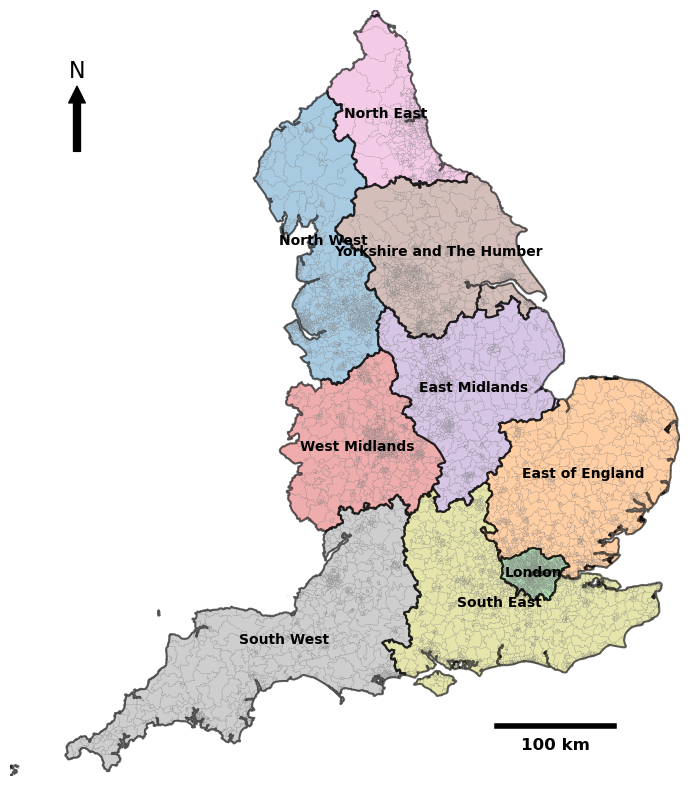
\includegraphics[width=.65\linewidth]{ucl-latex-thesis-templates-master/Image/datageo_area_1.png}
  \caption{Map of England with the boundary of nine regions and MSOAs.}
  \label{fig:A3.1}
\end{figure}%


\section{Data Sources and Data Processing}
\label{sec:3.2}
\subsection{DM prevalence}
\label{sec:3.2.1}
Our dependent variable, the MSOA-level DM prevalence data, is based on a project by Baker (2021). This project used a modeling approach to convert the prevalence data for 21 health conditions, originally provided at the GP practice level in the QOF dataset, into area-level data. Their latest dataset provides information based on the 2022/23 QOF data (Baker, 2024). Unlike the traditional method of simply applying population-weighted approaches to QOF datasets, Baker’s project accounted for more complex realities, making the estimates more accurate. They considered differences between registered GP populations and resident populations, recognizing that certain areas often have populations not registered with local NHS GPs, such as city centers, university districts, prisons, and military bases. Additionally, they accounted for area variations in disease incidence by using health and disability data from census records to assign appropriate weights to each area. Efforts were also made to address missing data from a small number of GP practices and exclude special cases, such as patients living in Wales but registered with GPs in England. Therefore, we have used the data derived from their modeled estimates method rather than simply applying a population-weighting approach to the QOF GP-level data.

\subsection{Demographic data}
\label{sec:3.2.2}
The demographic factors considered in this project include gender, age, ethnicity, and population density. The 2021 Census data provides population numbers for ethnic groups (ONS, 2021), which includes five broad categories: White, Black, Asian, Mixed, and Other, along with their specific subgroups. We use these five broad categories and calculate the corresponding population percentages as variables for the ethnic groups. Additionally, the ONS provides the latest population estimates at the MSOA level (ONS, 2024), which include gender population estimates for each age. From this dataset, we can calculate the proportion of female population and the age group proportions. The age group classification in this study is based on the work of Pham et al. (2019) on the prevalence of T2DM across the UK, using ten-year intervals. Additionally, we made adjustments according to the QOF guidance for 2022/23, specifically DM indicator DM017 (NHS England, 2022), which states that records for DM patients only include those aged 17 and over. Therefore, our age group classification is as follows: 17-29, 30-39, 40-49, 50-59, 60-69, 70-79, and 80+.


\subsection{Index of Multiple Deprivation data}
\label{sec:3.2.3}
The literature review has already explained the definition of the IMD, its calculation method, and its components. Here, we will only discuss how we use IMD data in this study. We used the latest 2019 English IMD dataset (MHCLG, 2019). The IMD research report explains how the IMD, originally measured at the LSOA level, is aggregated to the MSOA level (MHCLG, 2019). By using the LSOA-to-MSOA lookup table (ONS, 2021), we can obtain the IMD score for each MSOA by summing the population-weighted scores of the LSOAs contained within each MSOA. Once the IMD scores for all MSOAs are calculated, they are ranked, with a rank of 1 indicating the most deprived. At the same time, the corresponding decile representation is provided. Figure \ref{fig:A3.2} compares IMD scores at the LSOA and MSOA levels. We can see that the IMD score at the LSOA level provides more detailed granularity, but the MSOA level still captures significant distribution patterns.

While many studies use the IMD score directly as a variable for social deprivation—for example, Levene et al. (2019) in their study on NHS practice payments—they sometimes transform the variable, complicating interpretation. However, the IMD research report recommends using the rank and decile rather than the score, as the score’s calculation is highly complex, involving weighting and index transformations. This leads to inflation at the most deprived end of the scale, making the IMD score difficult to interpret (MHCLG, 2019). Therefore, we use the IMD decile as a variable to assess the relative deprivation of small areas.

When handling categorical data in regression models, dummy variable encoding is typically used. However, the IMD decile, which is ordinal data, is quite unique. Lang et al. (2016), in their study on cardiovascular disease risk, also used IMD decile and treated it as a continuous variable. This approach retains the ranking property of the IMD while benefiting from the assumption of linear relationships, thereby increasing the statistical power of the analysis and reducing model complexity. Therefore, we also treat the IMD decile as a continuous variable.


\begin{figure}[ht]
\centering
\begin{subfigure}{.39\textwidth}
  \centering
  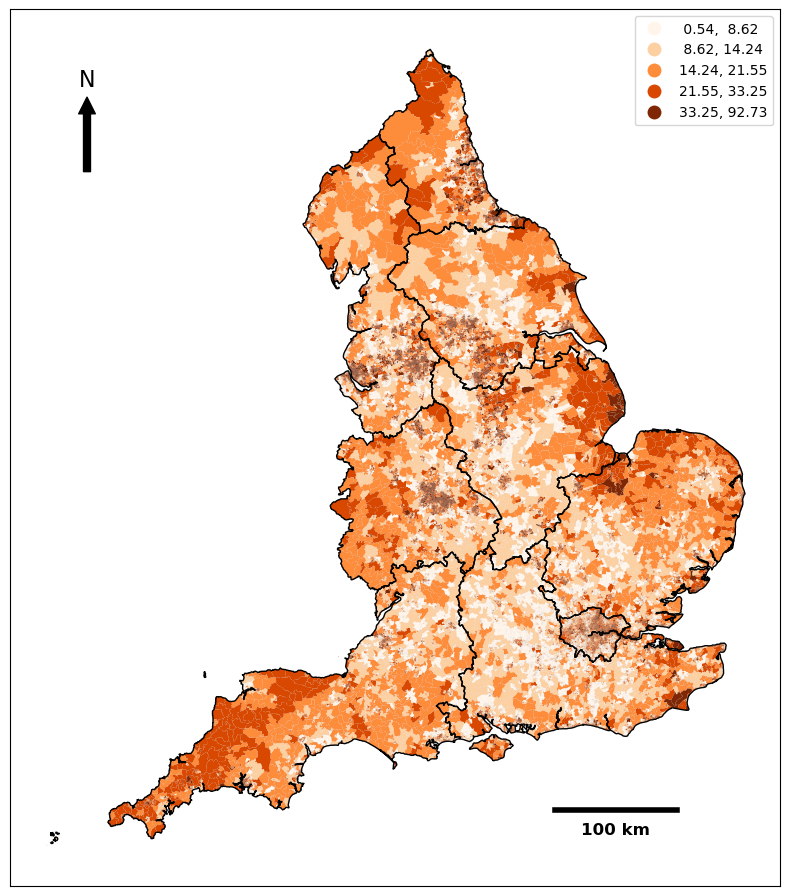
\includegraphics[width=1\linewidth]{ucl-latex-thesis-templates-master/Image/datageo_IMDLSOA_2.1.png}
  \caption{LSOA level.}
  \label{fig:A3.21}
\end{subfigure}%
\begin{subfigure}{.39\textwidth}
  \centering
  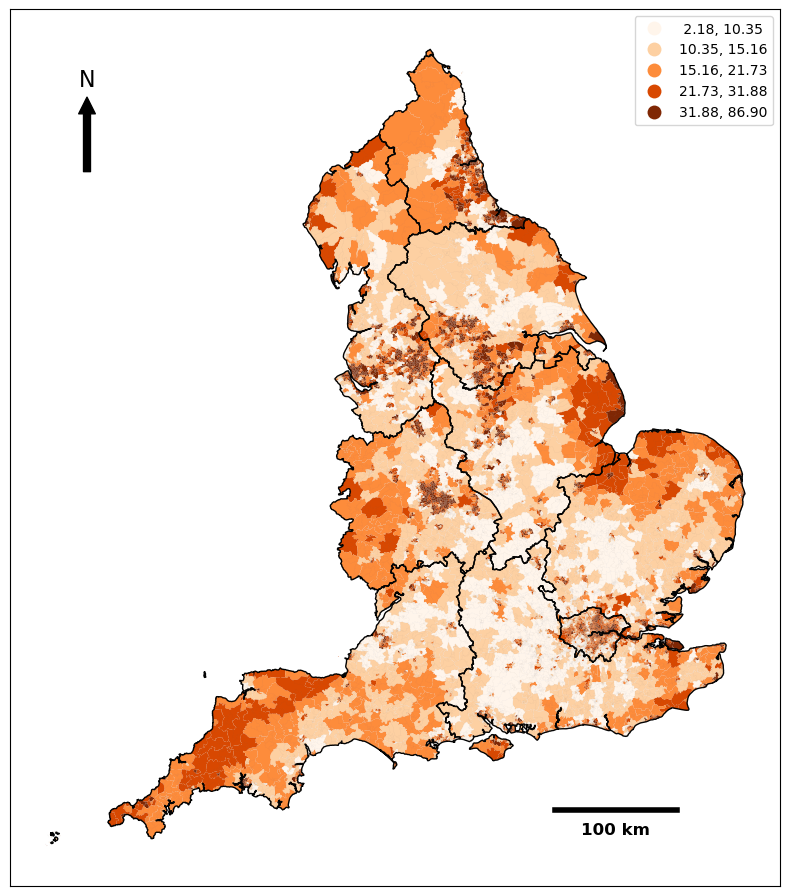
\includegraphics[width=1\linewidth]{ucl-latex-thesis-templates-master/Image/datageo_IMDMSOA_2.2.png}
  \caption{MSOA level.}
  \label{fig:A3.22}
\end{subfigure}
\caption{Maps comparing the geographical distribution of IMD scores at LSOA and MSOA levels.}
\label{fig:A3.2}
\end{figure}


\subsection{Lifestyle Group and Children Care}
\label{sec:3.2.4}
Based on the literature review, we found that unhealthy lifestyle habits such as drinking alcohol, smoking, and consuming sugary drinks are significant risk factors for diabetes. We collected corresponding datasets to represent variables in the lifestyle group. For alcohol misuse, we used the dataset provided by OHID, Hospital Admissions for Alcohol Attributable Conditions (2017), as a measure of alcohol abuse in different areas. This dataset calculates the standardized admission ratio for alcohol-related hospitalizations, with the numerator being alcohol-attributable admissions and the denominator being the expected number of admissions.
Smith et al. (2021) modeled dietary consumption among adults in England using small-area estimation methods. Their dataset, available at the MSOA level, aligns with our study's requirements. Their study focused on adults aged 16 and over, which matches our age group design. They calculated the average prevalence of adults consuming more than 330ml of sugar-sweetened beverages (SSBs) per day, a measure we will adopt.
For smoking behavior, we chose to use the prevalence of COPD, as Baker's project includes estimates of 20 health conditions, including COPD. According to NHS guidance (2022), around 90\% of COPD cases are smoking-related, with smoking being the primary cause. Given this strong correlation, we used COPD prevalence as an independent variable in the study, as it not only reflects smoking habits but also helps explore the connection between these two chronic conditions. Overweight status, another significant factor repeatedly mentioned in the literature, is measured at the MSOA level for obesity prevalence, also available from Baker's project. According to the OB002 indicator from the QOF 2022/23 guidance (NHS England, 2022), this obesity prevalence captures patients aged 18 and above with a BMI of 30 or higher, which fits our age group design.
We also included a variable reflecting child care using the Emergency admissions in children under five years old data provided by OHID (2023). This dataset calculates the number of completed emergency admissions as the numerator and the estimated population of children aged 0-4 as the denominator, multiplied by 1,000 to give a per-thousand rate. This dataset can highlight early health risk factors, helping us explore how early-life environments and childcare impact long-term health outcomes.


\subsection{Data Alignment for MSOA Boundary}
\label{sec:3.2.5}
It is important to note that our demographic variables are based on data from 2021 and beyond, using the 2021 MSOA boundaries. However, the other datasets, such as the 2019 IMD data, dietary studies using pre-2021 data, and various health data, all use the 2011 MSOA boundaries. Therefore, we standardized all datasets to the 2011 MSOA boundaries, as recalculating the other data to match the 2021 boundaries would be impractical due to the complexity of the calculations involved. The exact fit lookup file provided by ONS (2024) helps resolve this issue. The `CHNGIND’ column in the CSV file shows how the 2011 MSOAs were transformed into the 2021 MSOAs, categorizing the changes into four types: U (unchanged), S (split), M (merged), and X (mixed change). We found that 6,677 MSOAs remained unchanged. 75 2011 MSOAs were split into 155 2021 MSOAs, 32 were merged into 16, and 7 underwent complex changes, forming 8 2021 MSOAs. Using this lookup table, we can easily align our demographic dataset with the other datasets into a unified dataset.


\subsection{Project Code GitHub Repository}
\label{sec:3.2.6}
All the code for this project can be found at the following link: \url{https://github.com/ShengAric92/CASA0010_dissertation}, ensuring the reproducibility of the results. This project utilizes two programming languages, Python and R, for data processing, data analysis, and data visualization. The four Jupyter notebooks provided include `main\_data.ipynb', which demonstrates the entire data processing procedure, while the remaining notebooks display data visualization for each stage. Since the spatialreg package in R is highly effective for spatial regression analysis, R is used for data analysis in this project. Please refer to the `main\_methods\_spatial\_regression.qmd' file for details.


\section{Data Distribution}
\label{sec:3.3}
Figures \ref{fig:A3.3} and \ref{fig:A3.4}, respectively, show the histograms and Q-Q plots of all variables except the IMD decile to examine data distribution. We found that the variables within ethnic groups do not follow a normal distribution. Additionally, the following variables also do not conform to a normal distribution: Age17\_29, population density, children care (`Childrenemerg'), alcohol consumption (`Alcohol'), and high SSB consumption (`HighSSB'). Therefore, attention should be given to these variables in subsequent regression analyses, and appropriate data transformations, such as log transformation, may be necessary. The IMD decile variable is somewhat unique because deciles are a method that divides a distribution into ten equal parts, so it is not shown here. Furthermore, except for the IMD decile (considered as a continuous variable), population density (measured in people per hectare), `Childrenemerg', and `Alcohol', all other variables are expressed as percentages.

\begin{figure}[!ht]
  \centering
  
  % First figure
  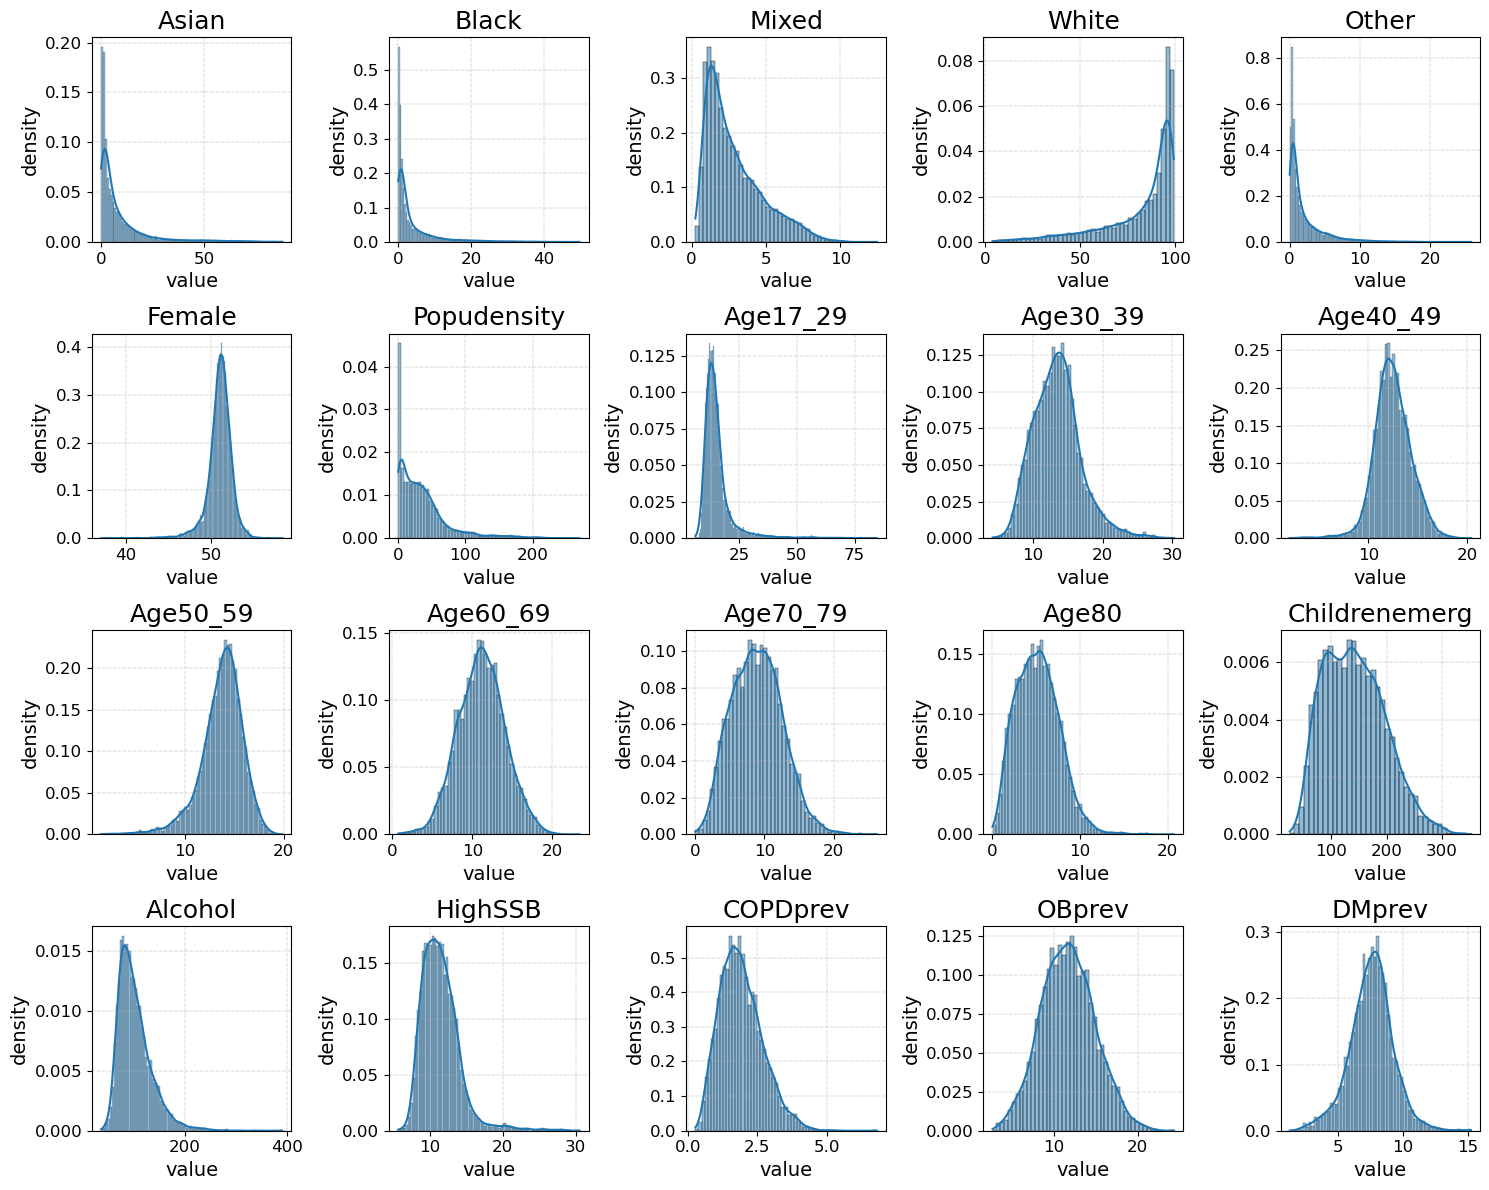
\includegraphics[width=.85\linewidth]{ucl-latex-thesis-templates-master/Image/data_hist_1.png}
  \caption{Histograms for All Variables (except IMD decile).}
  \label{fig:A3.3}
  
  \vspace{0.5cm} % Adjust vertical space between figures if needed
  
  % Second figure
  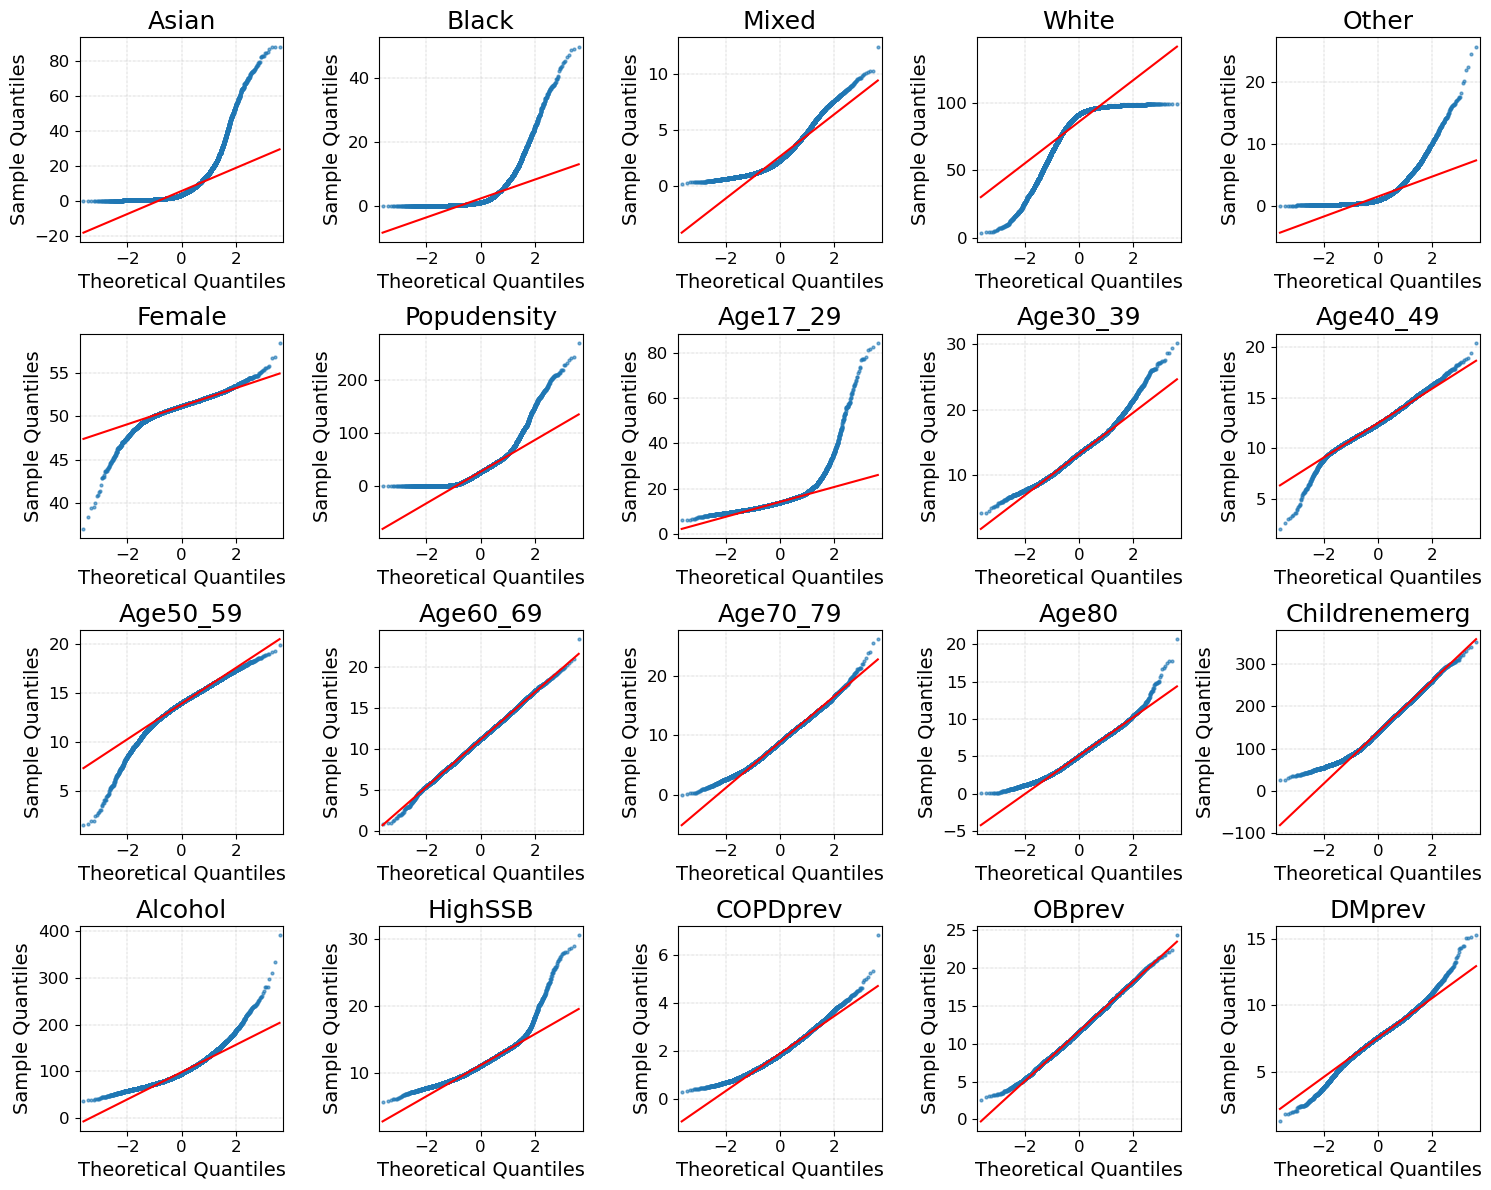
\includegraphics[width=.85\linewidth]{ucl-latex-thesis-templates-master/Image/data_qqplot_2.png}
  \caption{Q-Q Plots for All Variables (except IMD decile).}
  \label{fig:A3.4}
  
\end{figure}


\section{Methodology}
\label{sec:3.4}
To effectively address our research questions, this section will provide a methodology overview stage by stage.
\subsection{Exploratory Spatial Data Analysis}
\label{sec:3.4.1}
\subsubsection{Global Moran's I}
\label{sec:3.4.1.1}
Firstly, we need to explore the spatial distribution pattern of DM prevalence to determine whether it exhibits spatial clustering or dispersion. Therefore, the use of Global Moran's I is necessary, as it measures the degree of spatial autocorrelation of a variable across the entire study area. It is bounded by -1 and 1 and it is calculated using the form:
\begin{equation}
I=\frac{n}{s} \frac{\sum_{i=1}^n \sum_{j=1}^n w_{i j}\left(x_i-\bar{x}\right)\left(x_j-\bar{x}\right)}{\sum_{i=1}^n\left(x_i-\bar{x}\right)^2},
\end{equation}
where $n$ is the number of observations, $s$ is the sum of spatial weights, $\bar{x}$ is the mean of variable, and $w_{i j}$ denotes the spatial weight between observations index $i$ and $j$.

\subsubsection{Spatial Weights Matrix}
\label{sec:3.4.1.2}
This study uses Queen contiguity spatial weights to capture spatial interactions between neighboring areas. Given that the GP catchment areas at the MSOA level do not cover a large number of observations and that DM is a noncommunicable disease, which does not spread as rapidly as infectious diseases, K-Nearest Neighbours (KNN) spatial weights were ruled out. Additionally, the Isles of Scilly represent a special case, as the GP practice on the island provides medical services for the entire island. Thus, it is treated as an isolated unit and will employ a zero policy. Row normalization will be applied to meet the requirements for subsequent spatial dependence diagnostics and Monte Carlo Simulation.

\subsection{Correlation Analysis}
\label{sec:3.4.2}
Correlation analysis will be used to explore whether there is a linear relationship between variables. However, it’s important to remember that correlation does not imply causation. We will compute the Pearson correlation coefficient for each pair of variables to generate a sample correlation matrix. The entries of this matrix are defined by:

\begin{equation}
r_{i j}=\frac{\operatorname{cov}\left(v_i, v_j\right)}{\operatorname{sd}\left(v_i\right) * \operatorname{sd}\left(v_j\right)}=\frac{\sum_{l=1}^n\left(v_{i_l}-\bar{v}_i\right)\left(v_{j_l}-\bar{v}_j\right)}{\sqrt{\sum_{l=1}^n\left(v_{i_l}-\bar{v}_i\right)^2} \sqrt{\sum_{l=1}^n\left(v_{j_l}-\bar{v}_j\right)^2}},
\end{equation}
where $n$ is the size of observations, $v$ denotes the variable. IMD decile has been treated as a continuous variable, so it can also be used to calculate the Pearson correlation coefficient with other variables. Additionally, variables that are not significantly related to the dependent variable will be removed and excluded from the regression analysis.


\subsection{Regression Analysis: Ordinary Least Squares}
\label{sec:3.4.3}
\subsubsection{OLS Formula and Assumptions}
\label{sec:3.4.3.1}
To explore which risk factors significantly affect DM prevalence, we first established an Ordinary Least Squares (OLS) regression, with the following formula:
\begin{equation}
y=X \beta+\epsilon,
\end{equation}
where $y$ is the dependent variable, $X$ is the design matrix, $\beta$ is the vector of regression coefficients and $\epsilon$ is the error terms. In addition, the model must avoid multicollinearity and meet key assumptions, including homoscedasticity, independent errors, normally distributed errors, and exist a linear relationship. Therefore, the Durbin-Watson test, Jarque-Bera test, and Goldfeld-Quandt test will be used to assess whether the model meets these assumptions. Additionally, we use Z-score standardization to facilitate comparison between the regression coefficients.
\subsubsection{Variance Inflation Factor and Backward Elimination}
\label{sec:3.4.3.2}
In the age and ethnicity group variables, one variable from each group is manually removed as a reference variable to avoid multicollinearity. Additionally, the Variance Inflation Factor (VIF) is used to prevent multicollinearity, with a threshold set at 4 to avoid severe multicollinearity. To simplify the model, we also employed Backward Elimination (Marill and Green, 1963) to ensure that the remaining variables in the model are significant.
\subsubsection{Spatial Dependence Diagnostics}
\label{sec:3.4.3.3}
According to Anselin and Bera (1998), we know that OLS models are not always reliable because they do not account for spatial autocorrelation. Therefore, we need to perform spatial diagnostics on the OLS residuals, with Moran's I being used to test for spatial autocorrelation in the residuals. Suppose spatial autocorrelation is present in the residuals. In that case, we must then use spatial regression models such as the spatial lag model (SLM) or the spatial error model (SEM), and conduct Lagrange Multiplier (LM) tests and Robust LM tests to select the appropriate model. According to Anselin (2005), after performing the LM test, if either SLM or SEM is significant, the significant model should be chosen. If both models are significant, the Robust LM test is needed to select the appropriate model. If both models are significant in the Robust LM test, the model with the larger test statistic should be chosen.


\subsection{Spatial Regression Analysis}
\label{sec:3.4.4}
According to the studies by Osayomi (2019) and Turi (2017), three common spatial regression models are widely used in spatial epidemiology. These models are the spatial lag model (SLM), the spatial error model (SEM), and the spatial Durbin model (SDM). This subsection will introduce each of these three models.
\subsubsection{Spatial Lag Model}
\label{sec:3.4.4.1}
The SLM focuses on the spatial lag effect of the dependent variable, capturing whether the dependent variable in an area is influenced by the dependent variables in neighboring areas. Its formula is as follows:
\begin{equation}
y=\rho W y+X \beta+\epsilon.
\end{equation}
Here $\rho$ is the spatial lag coefficient, $W$ is the spatial weight matrix, $\beta$ is the regression coefficients vector and $\epsilon$ is the error term. $\rho W y$ is the added spatially lagged value, and due to the inclusion of this term, the SLM cannot be directly compared with OLS. Generally, we need to calculate the direct effect and the indirect effect in the model.
\subsubsection{Spatial Error Model}
\label{sec:3.4.4.2}
The SEM can handle spatial autocorrelation in the error terms. It can reveal clusters of unexplained spatially correlated values in neighbouring areas caused by omitted variables that were not included in the model. Its formula is as follows:
\begin{equation}
y=X \beta+u, \quad u=\lambda W u+\epsilon.
\end{equation}
Here $u$ is the function of unexplained residuals and neighbors residuals, where $\lambda$ measures the correlation between neighbouring residuals.
\subsubsection{Spatial Durbin Model}
\label{sec:3.4.4.3}
SLM and SEM can only capture part of the spatial dependency, whereas the SDM combines the considerations of both models. It can simultaneously capture the spatial lag effects of both the dependent and independent variables and helps to identify the spatial spillover effect of the independent variables, which is the impact of the independent variables in neighboring areas on the dependent variable in the current area. Its formula is:
\begin{equation}
y=\rho W y+X \beta+W X \theta+\epsilon.
\end{equation}
We need to note that the spatially lagged value of the independent variables is also included, where $\theta$ is the vector of spatially lagged independent variables' coefficients. Therefore, like the SLM, this model also requires the calculation of both the direct effect and the indirect effect of the variables.

\subsection{Model Selection and Comparison}
\label{sec:3.4.5}
\subsubsection{SDM Degenerate Test}
\label{sec:3.4.5.1}
Some economists and ecologists have started to expand the use of spatial regression models, suggesting that if both SLM and SEM remain highly significant after performing a Robust LM test, a more comprehensive model should be considered. For example, the studies by Patnaik (2023) and Shang (2024) used the Likelihood Ratio (LR) test to determine whether the SDM could degenerate into an SLM or SEM. If the LR test for both models is still highly significant with the SDM, it indicates that the SDM cannot be simplified to an SLM or SEM. Of course, the final choice should also consider the performance of these models and their relevance to real-world situations.
\subsubsection{Model Comparison}
\label{sec:3.4.5.2}
To compare the models, the Akaike Information Criterion (AIC) and the Bayesian Information Criterion (BIC) will be used. These two metrics assess the goodness of fit of the models, with lower AIC and BIC values indicating better model fit. Additionally, it is necessary to test for spatial autocorrelation in the model residuals, using Moran's I for diagnostic testing. If the model effectively removes spatial autocorrelation in the residuals, it indicates that the model has successfully captured and addressed the spatial dependencies in the data.

\section{Ethical evaluation}
\label{sec:3.5}
The ethical risk level of this project is considered minimal and does not require further ethical review, as all datasets used are openly available and can be easily downloaded free of charge. The data were sourced from various online platforms run by government agencies, such as demographic data from the ONS and public health data from NHS Digital and OHID. These datasets are provided under the Open Government Licence, the details of which can be found at this link: \url{https://www.nationalarchives.gov.uk/doc/open-government-licence/version/3/}. The availability of these data supports academic research, encourages innovation, and provides support and evidence for the development of public health policy.

This project also utilizes data based on research and other research projects. For example, Smith et al. (2021) estimated fruit, vegetable, and SSB consumption data in their study on adult dietary habits in England. Baker's project (2021) transformed the QOF's publicly available GP-level prevalence data for various conditions into estimated area-level prevalence data. The datasets produced by these two projects are available under the Creative Commons Attribution License (details here: \url{https://creativecommons.org/licenses/by/4.0/}) and the Open Parliament Licence (details here: \url{https://www.parliament.uk/site-information/copyright-parliament/open-parliament-licence/}), respectively. By making their research findings available online as open data, they uphold academic transparency and facilitate further research and reuse of the data. This aligns with the core values of transparency and inclusivity in health data science, as highlighted by Ford et al. (2019). This project has used these datasets correctly and cautiously, with careful and appropriate citation.

It is important to note that the method for estimating prevalence rates incorporates data on the distribution of patients at the LSOA level, publicly provided by the NHS for each GP. Since January 2020, the NHS has published quarterly reports on the distribution of GP patients (NHS England, 2020). The NHS ensures that these data are anonymized and do not include any patient address information, which aligns with Tene and Polonetsky's (2012) emphasis on balancing individual privacy with the beneficial use of data. Accordingly, this project's datasets and analyses do not involve personal or sensitive information.
\chapter{Results}
\label{chap:4}
\section{Exploratory Spatial Data Analysis}
\label{chap:4.1}
Figure \ref{fig:A4.1} shows the distribution of DM prevalence across nine regions and IMD deciles. We observe that the North East has the highest median prevalence, followed by the West Midlands. The South East has the lowest, with London coming in second-lowest. Interestingly, although the East Midlands contains the MSOA with the highest prevalence, it ranks only fourth overall. While the North East doesn’t have any areas exceeding 12\% prevalence, the distribution is fairly concentrated, indicating that most MSOAs in this region have a relatively high prevalence. On the other hand, London’s distribution is more spread out, suggesting greater variation in prevalence and potential health inequalities within the city. Based on IMD deciles, we can see that as the IMD decile increases (indicating less deprivation), DM prevalence gradually decreases. This aligns with our previous assumption that there is a linear relationship between IMD decile and DM prevalence, where less deprived areas tend to have lower prevalence.

\begin{figure}[ht]
\centering
\begin{subfigure}{.50\textwidth}
  \centering
  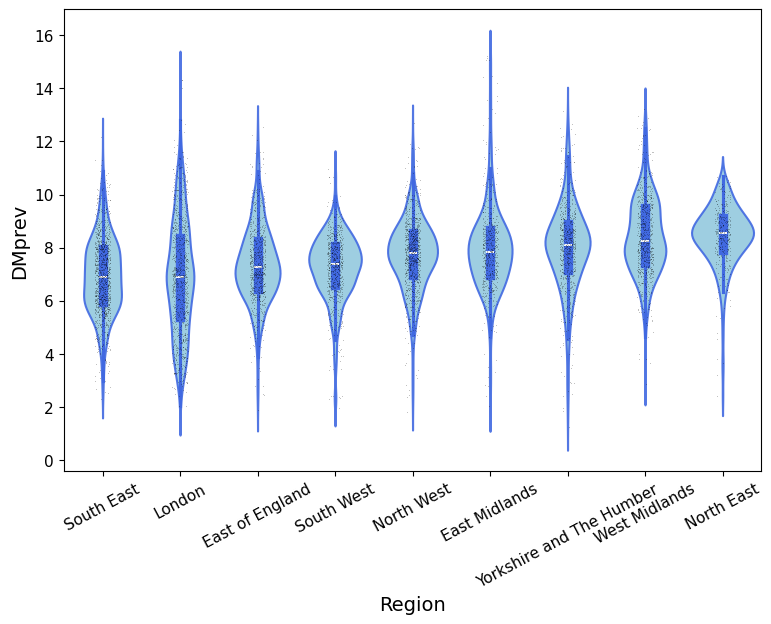
\includegraphics[width=1\linewidth]{ucl-latex-thesis-templates-master/Image/datageo_violin_3.1.png}
  \caption{Regions and DM prevalence.}
  \label{fig:A4.11}
\end{subfigure}%
\begin{subfigure}{.50\textwidth}
  \centering
  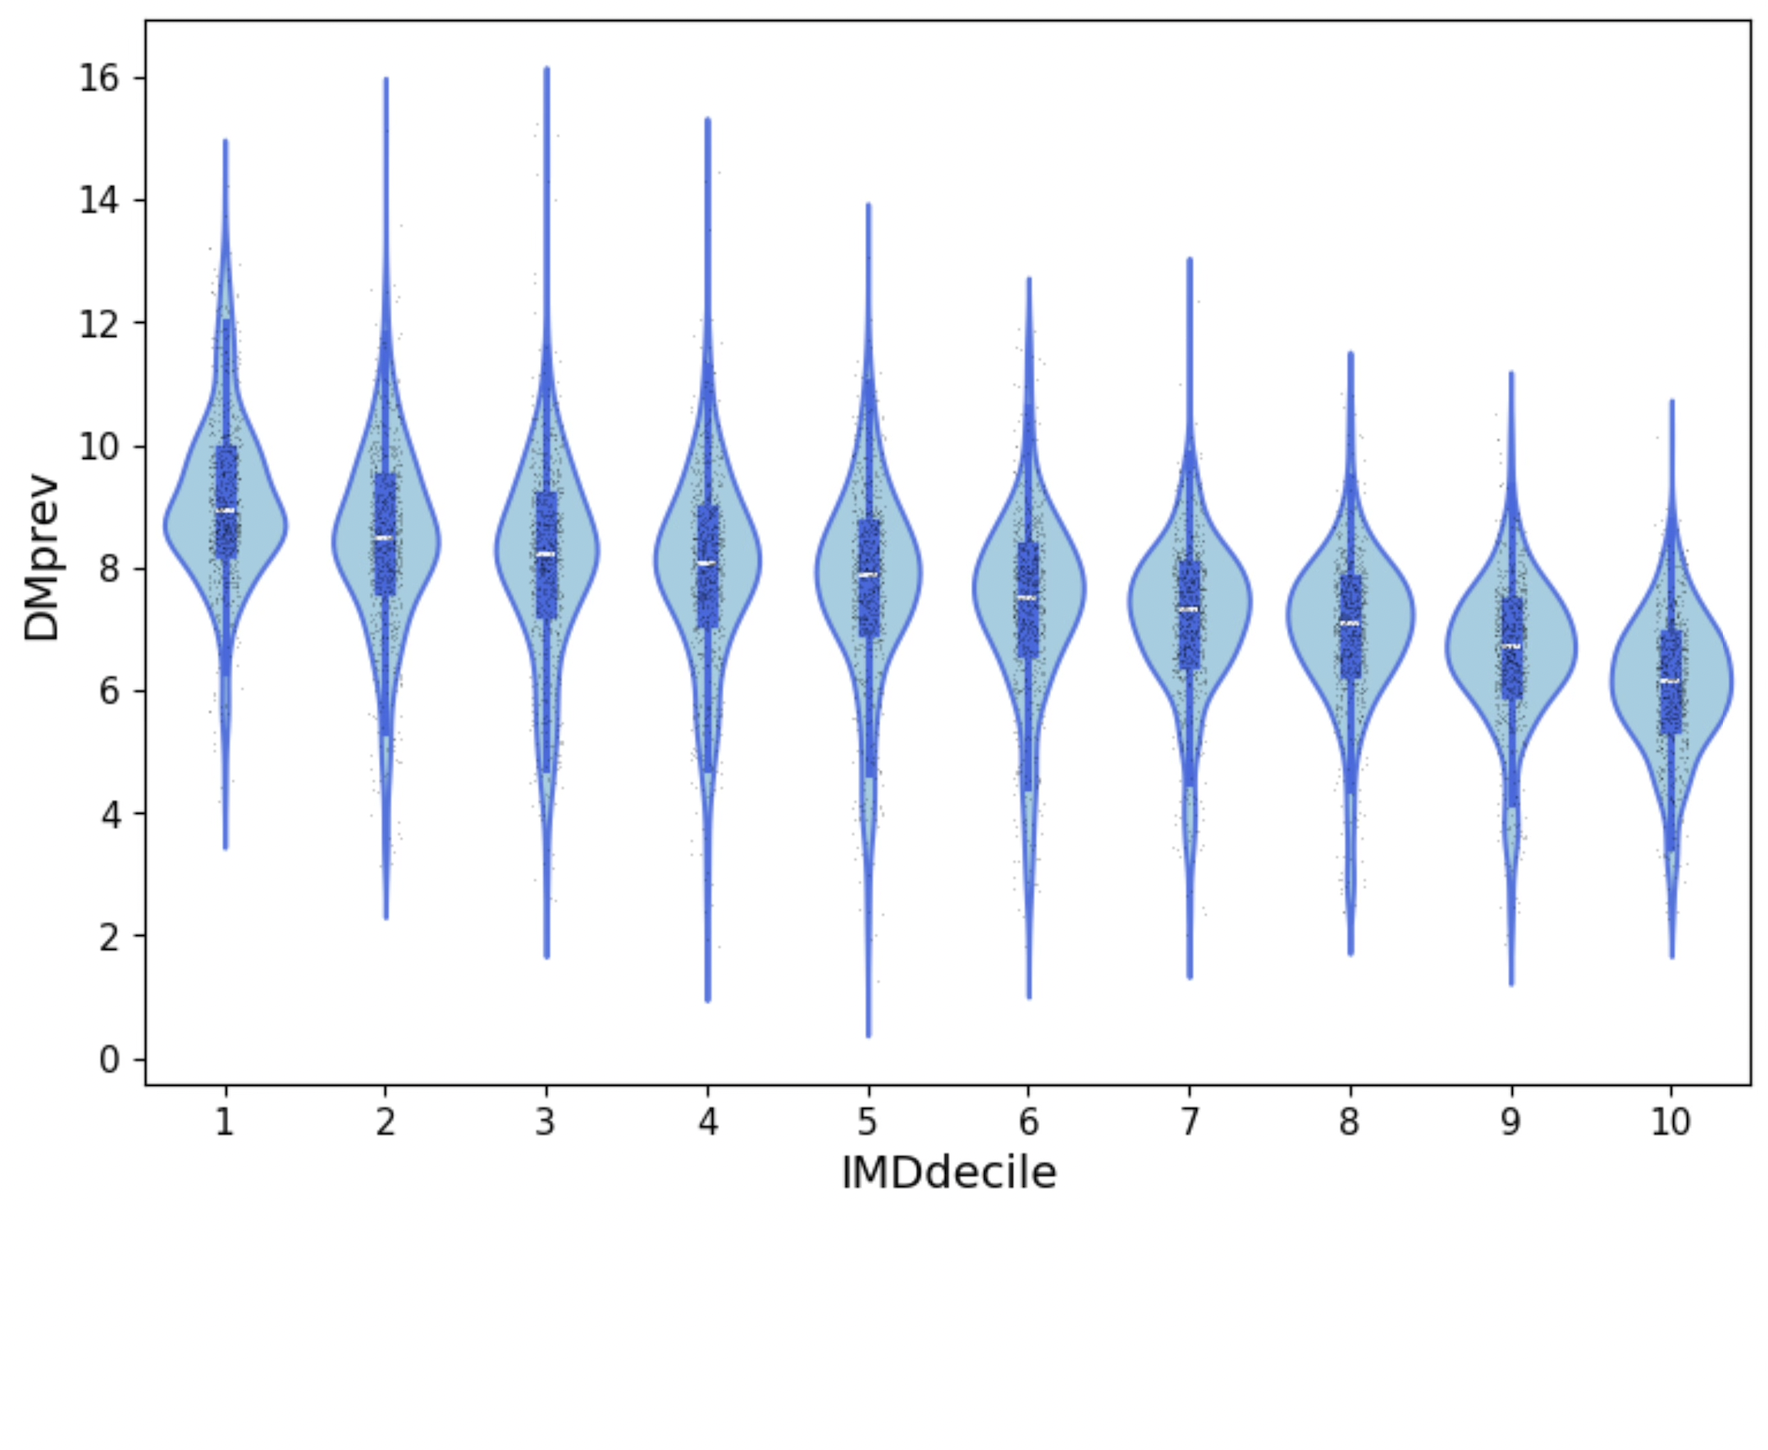
\includegraphics[width=1\linewidth]{ucl-latex-thesis-templates-master/Image/datageo_violin_3.2.png}
  \caption{IMD decile and DM prevalence.}
  \label{fig:A4.12}
\end{subfigure}
\caption{Violin plots for DM prevalence across nine regions and IMD deciles.}
\label{fig:A4.1}
\end{figure}

Figure \ref{fig:A4.2} shows the geographical distribution of DM prevalence. A Moran’s I statistic as high as 0.793 indicates a strong degree of spatial clustering. From the map, it’s evident that areas with very high DM prevalence are concentrated in the southern part of the North East, the eastern part of the East Midlands, and the northern part of the East of England. However, it’s interesting to note that despite this, the East of England has a median DM prevalence that ranks only the third-lowest out of the nine regions. We can also observe that cities like Oxford, Cambridge, and York have very low DM prevalence. In contrast, central England, including areas around cities like Birmingham, Nottingham, Sheffield, and Leeds, shows higher DM prevalence in the surrounding MSOAs.

Based on a review of the literature, I selected several risk factors that most scholars have emphasized, including obesity prevalence, IMD, and the Asian population, and mapped their geographical distribution (see Figure \ref{fig:A4.3}). We can see that the spatial distribution of obesity prevalence closely mirrors that of DM prevalence. IMD also shows a similar pattern, though to a slightly lesser extent. A common feature is that areas south of Grimsby exhibit both high DM and obesity prevalence, as well as high levels of deprivation. The Asian population, however, displays a different spatial pattern, concentrating around major cities. However, coincidentally, the MSOAs around these cities also tend to have a very high DM prevalence.


\begin{figure}[ht]
  \centering
  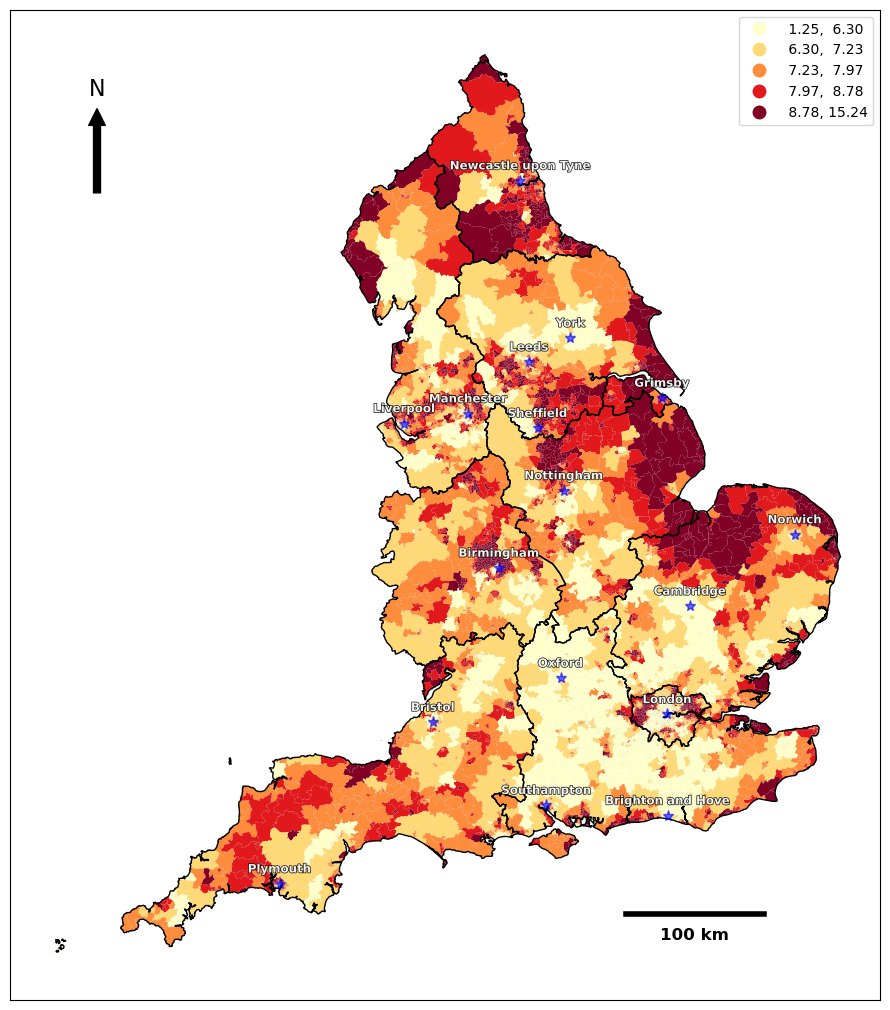
\includegraphics[width=.99\linewidth]{ucl-latex-thesis-templates-master/Image/datageo_DMprev_4.png}
  \caption{Geographical distribution of DM prevalence.}
  \label{fig:A4.2}
\end{figure}%


\begin{figure}[ht]
\centering
\begin{subfigure}{.4\textwidth}
  \centering
  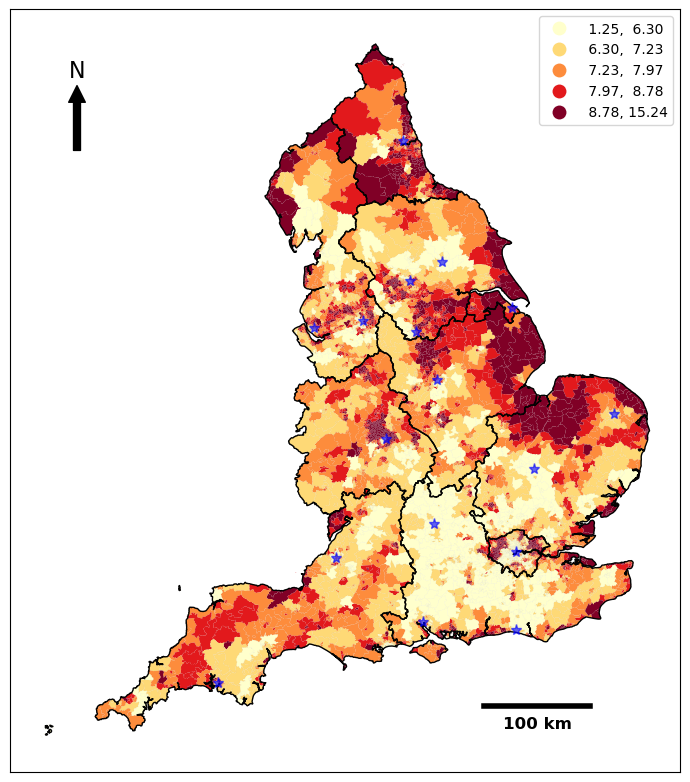
\includegraphics[width=1\linewidth]{ucl-latex-thesis-templates-master/Image/datageo_DMprev_5.png}
  \caption{DM prevalence.}
  \label{fig:A4.31}
\end{subfigure}%
\begin{subfigure}{.4\textwidth}
  \centering
  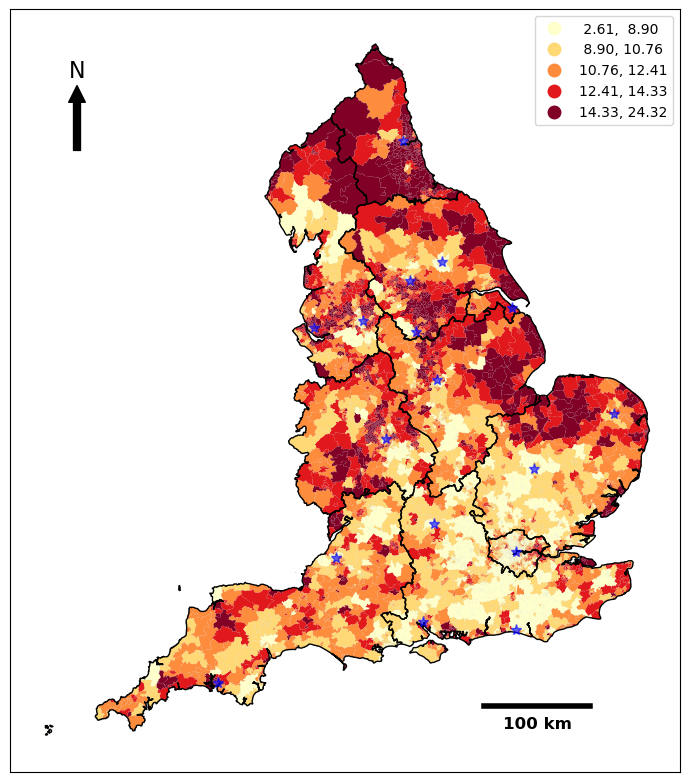
\includegraphics[width=1\linewidth]{ucl-latex-thesis-templates-master/Image/datageo_OBprev_6.png}
  \caption{Obesity prevalence.}
  \label{fig:A4.32}
\end{subfigure}
\begin{subfigure}{.4\textwidth}
  \centering
  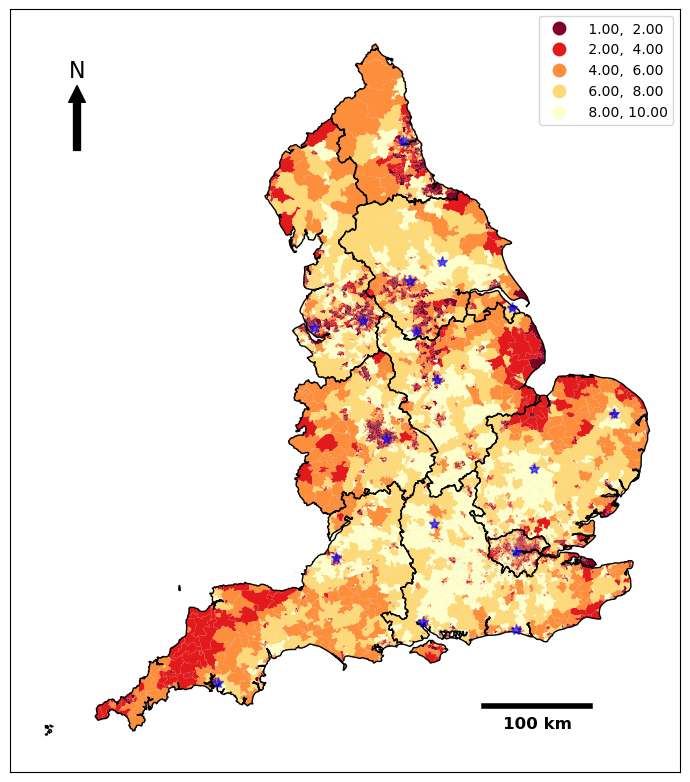
\includegraphics[width=1\linewidth]{ucl-latex-thesis-templates-master/Image/datageo_IMDdecile_7.png}
  \caption{IMD.}
  \label{fig:A4.33}
\end{subfigure}
\begin{subfigure}{.4\textwidth}
  \centering
  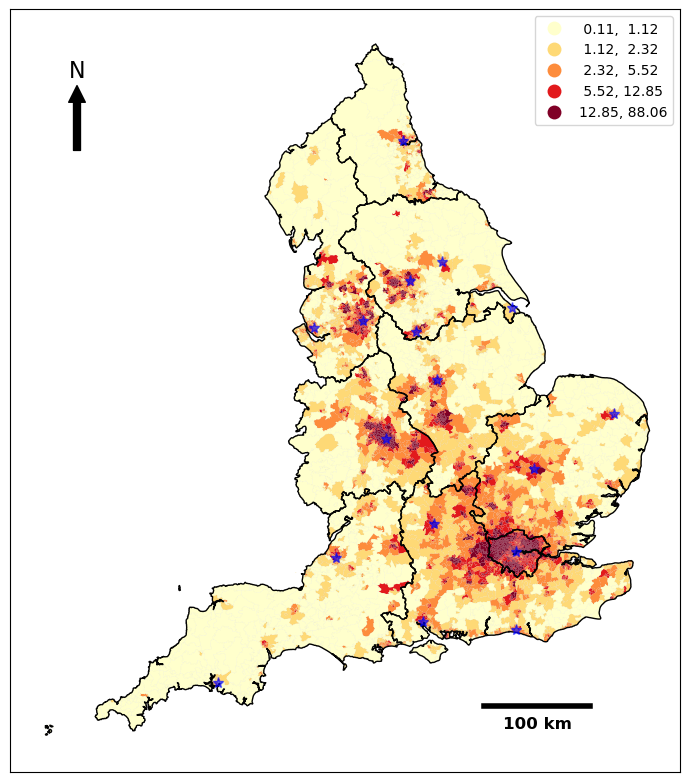
\includegraphics[width=1\linewidth]{ucl-latex-thesis-templates-master/Image/datageo_Asian_8.png}
  \caption{Asian population.}
  \label{fig:A4.34}
\end{subfigure}
\caption{Maps of selected variables.}
\label{fig:A4.3}
\end{figure}

\clearpage
\section{Correlation Analysis}
\label{chap:4.2}
Figure \ref{fig:A4.4} presents the correlation scatter plots between all independent variables and DM prevalence. Given the large number of observations, all independent variables show a significant correlation with DM prevalence, meaning no variables were eliminated at this stage. Among the ethnic groups, we observe a moderate positive correlation between the Asian population and DM prevalence, while Mixed, White, and Other populations all show a negative correlation with DM prevalence. Age17\_29 exhibits a clear negative linear relationship in the age groups, whereas Age60\_69 shows a positive linear relationship. Lifestyle factors and childcare are also positively correlated with DM prevalence, except for HighSSB. Figure \ref{fig:A4.5} displays the heat map of the correlation matrix, revealing what appears to be high multicollinearity among the independent variables.

\begin{figure}[ht]
  \centering
  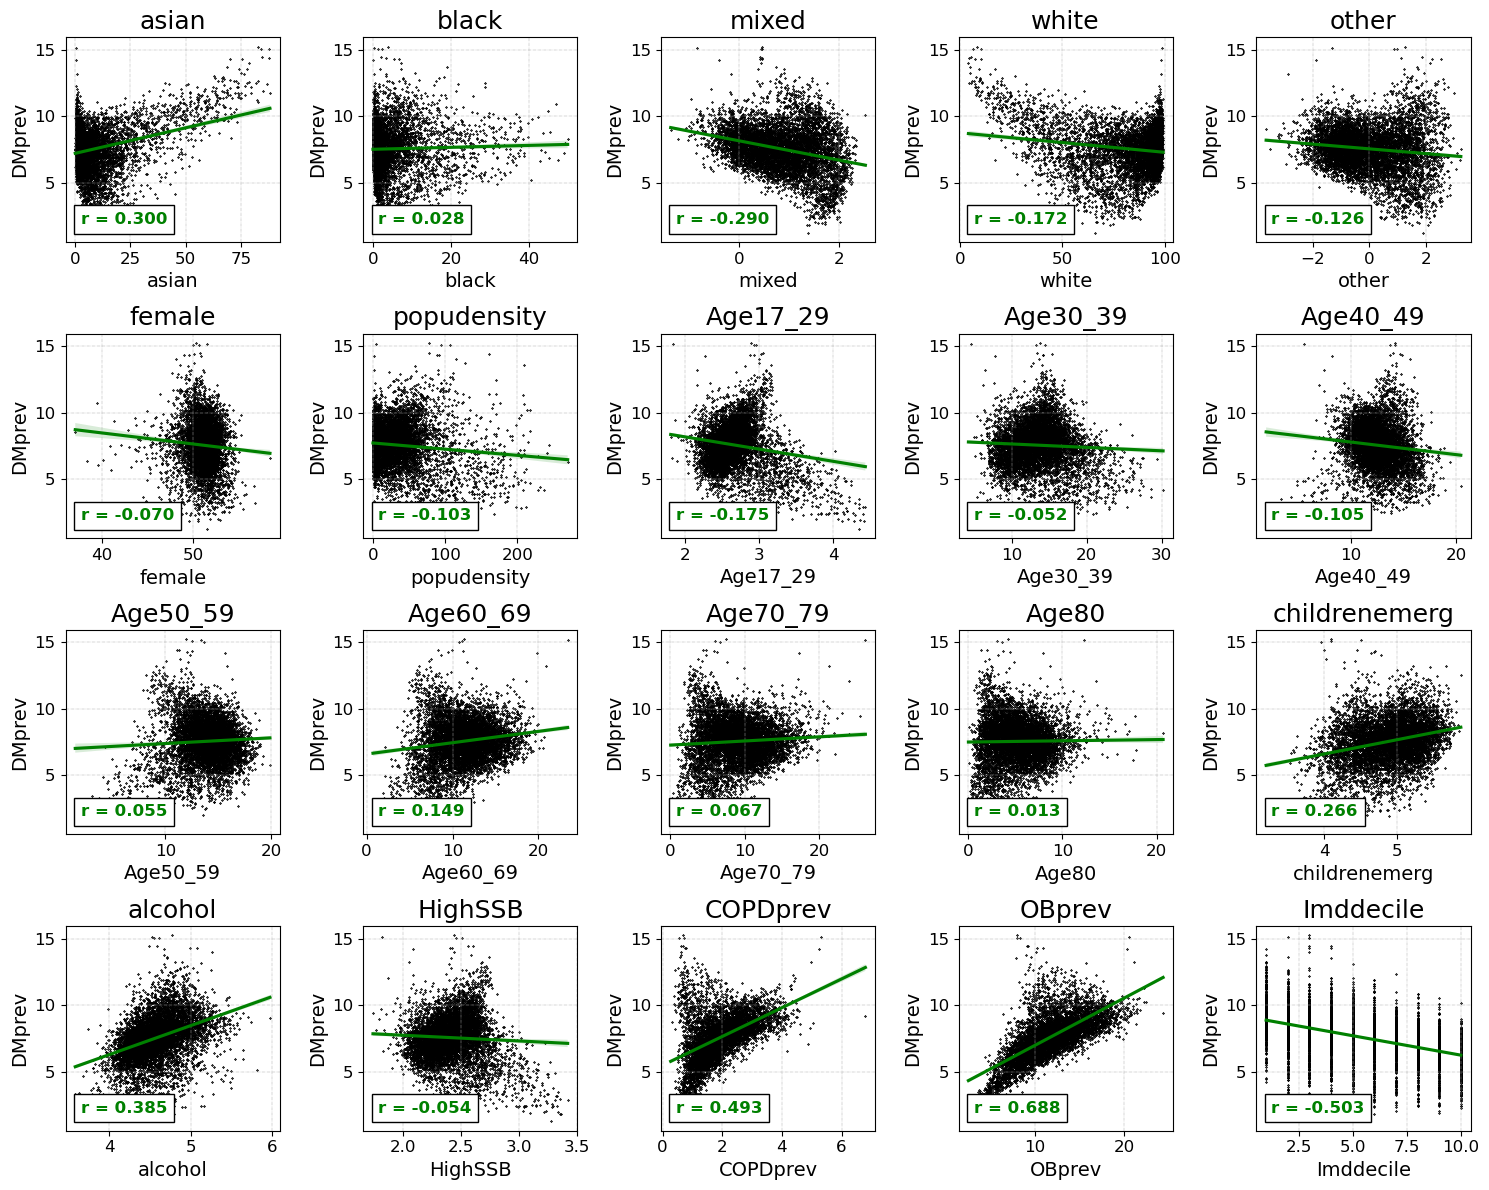
\includegraphics[width=.99\linewidth]{ucl-latex-thesis-templates-master/Image/methods_corrscat_1.png}
  \caption{Scatter plots of DM prevalence vs all explanatory variables.}
  \label{fig:A4.4}
\end{figure}%

\vspace{10pt}

\begin{figure}[ht]
  \centering
  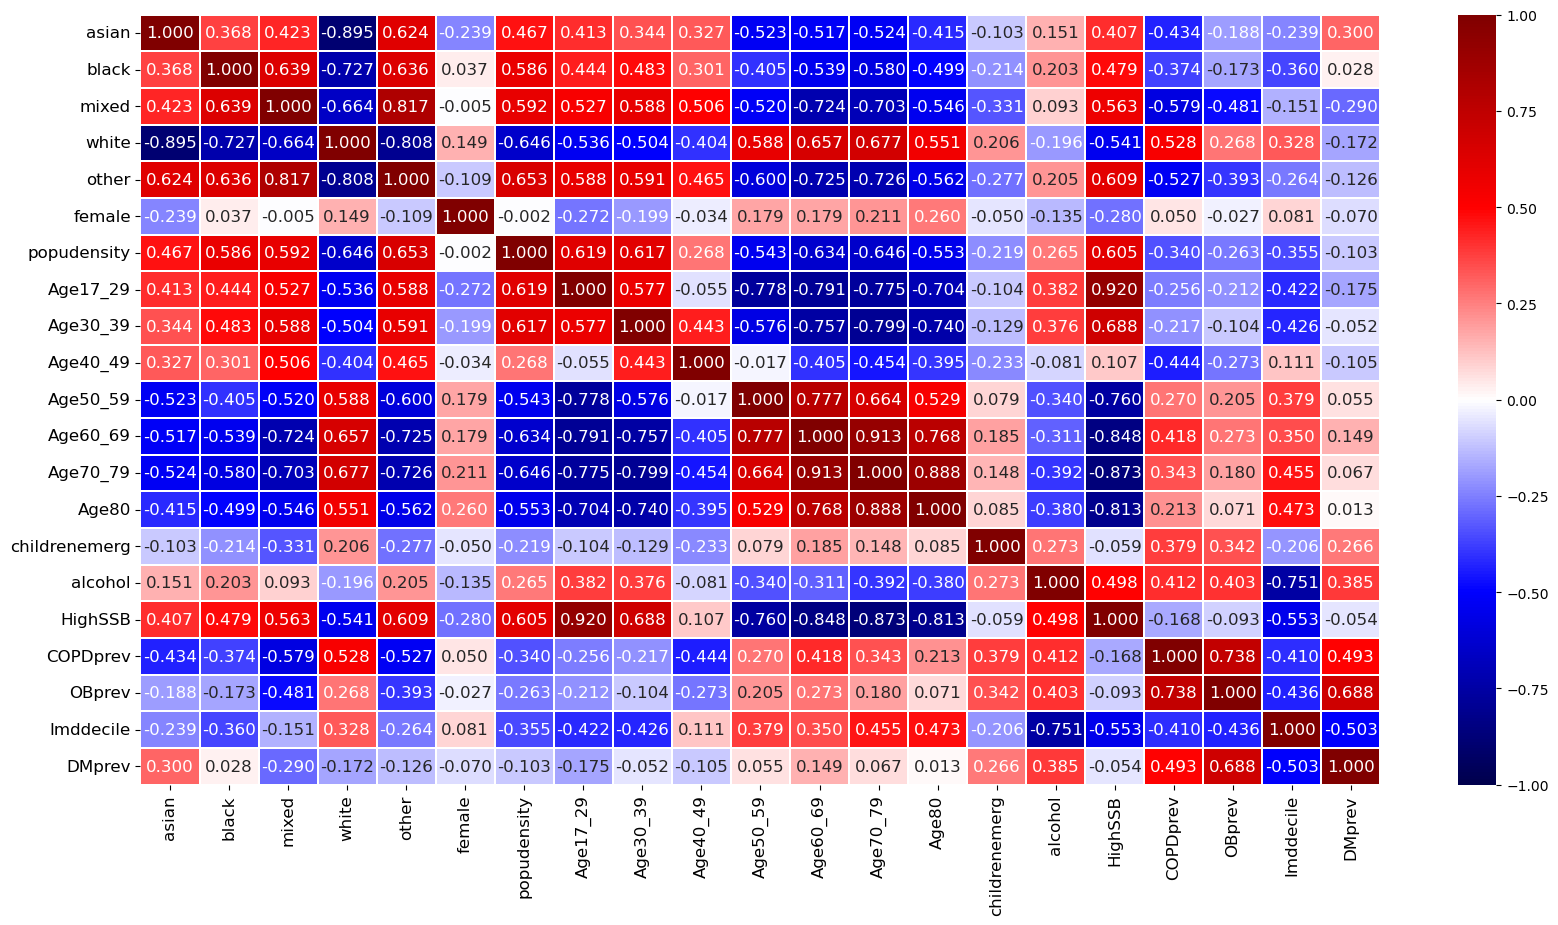
\includegraphics[width=.99\linewidth]{ucl-latex-thesis-templates-master/Image/methods_corrmatrix_2.png}
  \caption{Heat map of the correlation matrix.}
  \label{fig:A4.5}
\end{figure}%



\section{Ordinary Least Squares}
\label{chap:4.3}
We manually removed the two most prevalent variables from the age and ethnicity groups, Age17\_29 and White population, to avoid multicollinearity.
Table \ref{tab: A4.1} presents our initial OLS model based on a selection criterion of VIF < 4. Among the remaining variables, only Age30\_39, Children care, and Alcohol are not significant, while the others are significant. Since the data has been standardized, the coefficients can be compared. The top three contributing factors are the Asian population, obesity prevalence, and IMD decile. With an R-squared of 0.7613, the model demonstrates strong explanatory power, indicating that the independent variables account for 76.13\% of the variation in DM prevalence.
Table \ref{tab: A4.2} presents the OLS model after Backward Elimination, with a slight reduction in AIC without significantly affecting the R-squared. This suggests that Backward Elimination successfully removed the three non-significant variables, reducing model complexity without compromising its explanatory capacity.
Although the Jarque-Bera test's p-value is highly significant, indicating that the residuals of the model do not meet the assumption of normality due to the large number of observations, the Central Limit Theorem applies, allowing us to relax this assumption. Figure \ref{fig:A4.6} shows that, despite the significance of the Jarque-Bera test, the histogram of the residuals still largely follows a normal distribution, as expected under the Central Limit Theorem.
Table \ref{tab: A4.3} highlights that the residuals of the OLS model exhibit significant spatial autocorrelation, with a high Moran's I statistic of 0.573, indicating the need for spatial regression models. The LM diagnostics results shown in Table \ref{tab: A4.4} indicate that both the LM Lag and LM Error tests are significant. Additionally, the Robust LM tests for both models are also significant. Although the Robust LM Error statistic is larger (1674.75) than the Robust LM Lag (487.13), suggesting the use of an SEM, the significance of both statistics means that a more comprehensive SDM should also be considered.

%%%%%%%
%%%%%%% OLS VIF
%%%%%%%
\begin{table}[]
\centering
\begin{tabular}{|llllll|}
\hline
\multicolumn{1}{|l|}{\textbf{Variable}} & \multicolumn{1}{l|}{\textbf{Coefficient}} & \multicolumn{1}{l|}{\textbf{Std. Error}} & \multicolumn{1}{l|}{\textbf{P-value}} & \multicolumn{1}{l|}{\textbf{Significance}} & \textbf{VIF} \\ \hline
\multicolumn{1}{|l|}{(Intercept)}       & \multicolumn{1}{l|}{1.250e-15}            & \multicolumn{1}{l|}{0.005935}                    & \multicolumn{1}{l|}{1.00000}          & \multicolumn{1}{l|}{}                      & /            \\ \hline
\multicolumn{1}{|l|}{Asian}             & \multicolumn{1}{l|}{0.5560}               & \multicolumn{1}{l|}{0.008316}                    & \multicolumn{1}{l|}{\textless 2e-16}  & \multicolumn{1}{l|}{***}                   & 1.963303     \\ \hline
\multicolumn{1}{|l|}{Black}             & \multicolumn{1}{l|}{0.1228}               & \multicolumn{1}{l|}{0.008653}                    & \multicolumn{1}{l|}{\textless 2e-16}  & \multicolumn{1}{l|}{***}                   & 2.125326     \\ \hline
\multicolumn{1}{|l|}{Mixed}             & \multicolumn{1}{l|}{-0.1612}              & \multicolumn{1}{l|}{0.01100}                    & \multicolumn{1}{l|}{\textless 2e-16}  & \multicolumn{1}{l|}{***}                   & 3.434716     \\ \hline
\multicolumn{1}{|l|}{Female}            & \multicolumn{1}{l|}{0.0238}               & \multicolumn{1}{l|}{0.006665}                    & \multicolumn{1}{l|}{0.00036}          & \multicolumn{1}{l|}{***}                   & 1.260857     \\ \hline
\multicolumn{1}{|l|}{Popudensity}       & \multicolumn{1}{l|}{-0.1470}              & \multicolumn{1}{l|}{0.009263}                    & \multicolumn{1}{l|}{\textless 2e-16}  & \multicolumn{1}{l|}{***}                   & 2.435609     \\ \hline
\multicolumn{1}{|l|}{Age30\_39}         & \multicolumn{1}{l|}{0.01117}              & \multicolumn{1}{l|}{0.01119}                    & \multicolumn{1}{l|}{0.31801}          & \multicolumn{1}{l|}{}                      & 3.554550     \\ \hline
\multicolumn{1}{|l|}{Age40\_49}         & \multicolumn{1}{l|}{0.05527}              & \multicolumn{1}{l|}{0.009273}                    & \multicolumn{1}{l|}{2.64e-09}         & \multicolumn{1}{l|}{***}                   & 2.440698     \\ \hline
\multicolumn{1}{|l|}{Age50\_59}         & \multicolumn{1}{l|}{0.1439}               & \multicolumn{1}{l|}{0.009989}                    & \multicolumn{1}{l|}{\textless 2e-16}  & \multicolumn{1}{l|}{***}                   & 2.832384     \\ \hline
\multicolumn{1}{|l|}{Age80}             & \multicolumn{1}{l|}{0.2001}               & \multicolumn{1}{l|}{0.01001}                    & \multicolumn{1}{l|}{\textless 2e-16}  & \multicolumn{1}{l|}{***}                   & 2.841857     \\ \hline
\multicolumn{1}{|l|}{Childrenemerg}     & \multicolumn{1}{l|}{0.002875}             & \multicolumn{1}{l|}{0.006747}                    & \multicolumn{1}{l|}{0.67000}          & \multicolumn{1}{l|}{}                      & 1.292357     \\ \hline
\multicolumn{1}{|l|}{Alcohol}           & \multicolumn{1}{l|}{0.004924}             & \multicolumn{1}{l|}{0.009511}                    & \multicolumn{1}{l|}{0.60470}          & \multicolumn{1}{l|}{}                      & 2.567739     \\ \hline
\multicolumn{1}{|l|}{OBprev}            & \multicolumn{1}{l|}{0.5276}               & \multicolumn{1}{l|}{0.008856}                    & \multicolumn{1}{l|}{\textless 2e-16}  & \multicolumn{1}{l|}{***}                   & 2.226523     \\ \hline
\multicolumn{1}{|l|}{IMDdecile}         & \multicolumn{1}{l|}{-0.3203}              & \multicolumn{1}{l|}{0.01126}                    & \multicolumn{1}{l|}{\textless 2e-16}  & \multicolumn{1}{l|}{***}                   & 3.597933     \\ \hline \hline
\multicolumn{6}{|l|}{\textbf{Multiple R-squared:} 0.7613}                                                                                                                                        \\ \hline
\multicolumn{6}{|l|}{\textbf{Adjusted R-squared:} 0.7608}                                                                                                                                        \\ \hline
\multicolumn{6}{|l|}{\textbf{F-statistic:} 1662.29}                                                                                                                                              \\ \hline
\multicolumn{6}{|l|}{\textbf{F-statistic p value:} \textless 2.2e-16}                                                                                                                            \\ \hline
\multicolumn{6}{|l|}{\textbf{Log-Likelihood:} -4771.83}                                                                                                                                          \\ \hline
\multicolumn{6}{|l|}{\textbf{AIC:} 9573.66}                                                                                                                                                      \\ \hline
\multicolumn{6}{|l|}{\textbf{BIC:} 9676.01}                                                                                                                                                      \\ \hline
\multicolumn{6}{|l|}{\textbf{RMSE:} 0.4886}                                                                                                                                                      \\ \hline \hline
\multicolumn{6}{|l|}{\textbf{Durbin-Watson test:} 1.0012}                                                                                                                                        \\ \hline
\multicolumn{6}{|l|}{\textbf{Jarque-Bera test p value:} \textless 2.2e-16}                                                                                                                       \\ \hline
\multicolumn{6}{|l|}{\textbf{Goldfeld-Quandt test p value:} 0.3094}                                                                                                                              \\ \hline \hline
\multicolumn{6}{|l|}{\textbf{Significance codes:} 0 ‘***’ 0.001 ‘**’ 0.01 ‘*’ 0.05 ‘.’ 0.1 ‘ ’ 1}                                                                                                \\ \hline
\end{tabular}
\caption{
The summary statistics of the initial OLS model.
}
\label{tab: A4.1}
\end{table}


%%%%%%%
%%%%%%% OLS Stepwise
%%%%%%%
\clearpage
\begin{table}[]
\centering
\begin{tabular}{|llllll|}
\hline
\multicolumn{1}{|l|}{\textbf{Variable}} & \multicolumn{1}{l|}{\textbf{Coefficient}} & \multicolumn{1}{l|}{\textbf{Std. Error}} & \multicolumn{1}{l|}{\textbf{P-value}} & \multicolumn{1}{l|}{\textbf{Significance}} & \textbf{VIF} \\ \hline
\multicolumn{1}{|l|}{(Intercept)}       & \multicolumn{1}{l|}{1.807e-15}            & \multicolumn{1}{l|}{0.005934} & \multicolumn{1}{l|}{1.00000}          & \multicolumn{1}{l|}{}                      & /            \\ \hline
\multicolumn{1}{|l|}{Asian}             & \multicolumn{1}{l|}{0.5529}               & \multicolumn{1}{l|}{0.007853} & \multicolumn{1}{l|}{\textless 2e-16}  & \multicolumn{1}{l|}{***}                   & 1.750827     \\ \hline
\multicolumn{1}{|l|}{Black}             & \multicolumn{1}{l|}{0.1216}               & \multicolumn{1}{l|}{0.008577} & \multicolumn{1}{l|}{\textless 2e-16}  & \multicolumn{1}{l|}{***}                   & 2.088520     \\ \hline
\multicolumn{1}{|l|}{Mixed}             & \multicolumn{1}{l|}{-0.1608}              & \multicolumn{1}{l|}{0.01086} & \multicolumn{1}{l|}{\textless 2e-16}  & \multicolumn{1}{l|}{***}                   & 3.348141     \\ \hline
\multicolumn{1}{|l|}{Female}            & \multicolumn{1}{l|}{0.02237}              & \multicolumn{1}{l|}{0.006552} & \multicolumn{1}{l|}{0.000643}         & \multicolumn{1}{l|}{***}                   & 1.218749     \\ \hline
\multicolumn{1}{|l|}{Popudensity}       & \multicolumn{1}{l|}{-0.1444}              & \multicolumn{1}{l|}{0.008799} & \multicolumn{1}{l|}{\textless 2e-16}  & \multicolumn{1}{l|}{***}                   & 2.198365     \\ \hline
\multicolumn{1}{|l|}{Age40\_49}         & \multicolumn{1}{l|}{0.05928}              & \multicolumn{1}{l|}{0.008464} & \multicolumn{1}{l|}{2.72e-12}         & \multicolumn{1}{l|}{***}                   & 2.034045     \\ \hline
\multicolumn{1}{|l|}{Age50\_59}         & \multicolumn{1}{l|}{0.1394}               & \multicolumn{1}{l|}{0.009205} & \multicolumn{1}{l|}{\textless 2e-16}  & \multicolumn{1}{l|}{***}                   & 2.405596     \\ \hline
\multicolumn{1}{|l|}{Age80}             & \multicolumn{1}{l|}{0.1969}               & \multicolumn{1}{l|}{0.009474} & \multicolumn{1}{l|}{\textless 2e-16}  & \multicolumn{1}{l|}{***}                   & 2.548242     \\ \hline
\multicolumn{1}{|l|}{OBprev}            & \multicolumn{1}{l|}{0.5293}               & \multicolumn{1}{l|}{0.008710} & \multicolumn{1}{l|}{\textless 2e-16}  & \multicolumn{1}{l|}{***}                   & 2.153809     \\ \hline
\multicolumn{1}{|l|}{IMDdecile}         & \multicolumn{1}{l|}{-0.3259}              & \multicolumn{1}{l|}{0.009265} & \multicolumn{1}{l|}{\textless 2e-16}  & \multicolumn{1}{l|}{***}                   & 2.437461     \\ \hline \hline
\multicolumn{6}{|l|}{\textbf{Multiple R-squared:} 0.7612}                                                                                                                                        \\ \hline
\multicolumn{6}{|l|}{\textbf{Adjusted R-squared:} 0.7609}                                                                                                                                        \\ \hline
\multicolumn{6}{|l|}{\textbf{F-statistic:} 2161.28}                                                                                                                                              \\ \hline
\multicolumn{6}{|l|}{\textbf{F-statistic p value:} \textless 2.2e-16}                                                                                                                            \\ \hline
\multicolumn{6}{|l|}{\textbf{Log-Likelihood:} -4772.61}                                                                                                                                          \\ \hline
\multicolumn{6}{|l|}{\textbf{AIC:} 9569.23}                                                                                                                                                      \\ \hline
\multicolumn{6}{|l|}{\textbf{BIC:} 9651.11}                                                                                                                                                      \\ \hline
\multicolumn{6}{|l|}{\textbf{RMSE:} 0.4886}                                                                                                                                                      \\ \hline \hline
\multicolumn{6}{|l|}{\textbf{Durbin-Watson test:} 1.0029}                                                                                                                                        \\ \hline
\multicolumn{6}{|l|}{\textbf{Jarque-Bera test p value:} \textless 2.2e-16}                                                                                                                       \\ \hline
\multicolumn{6}{|l|}{\textbf{Goldfeld-Quandt test p value:} 0.2254}                                                                                                                              \\ \hline \hline
\multicolumn{6}{|l|}{\textbf{Significance codes:} 0 ‘***’ 0.001 ‘**’ 0.01 ‘*’ 0.05 ‘.’ 0.1 ‘ ’ 1}                                                                                                \\ \hline
\end{tabular}
\caption{
The summary statistics of the OLS model (after Backward Elimination).
}
\label{tab: A4.2}
\end{table}

\begin{figure}[!ht]
\centering
\begin{subfigure}{.45\textwidth}
  \centering
  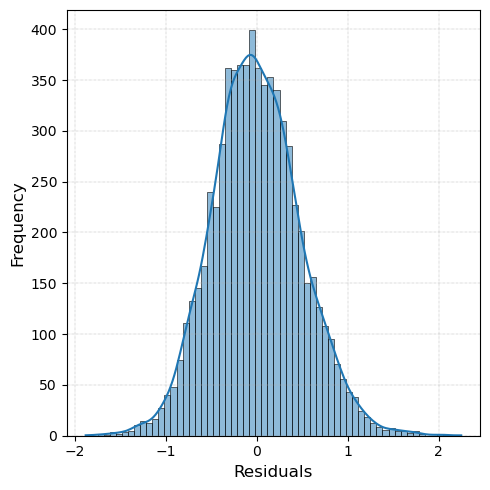
\includegraphics[width=1\linewidth]{ucl-latex-thesis-templates-master/Image/resi_OLS_1.1.png}
  \caption{Histogram.}
  \label{fig:A4.61}
\end{subfigure}%
\begin{subfigure}{.45\textwidth}
  \centering
  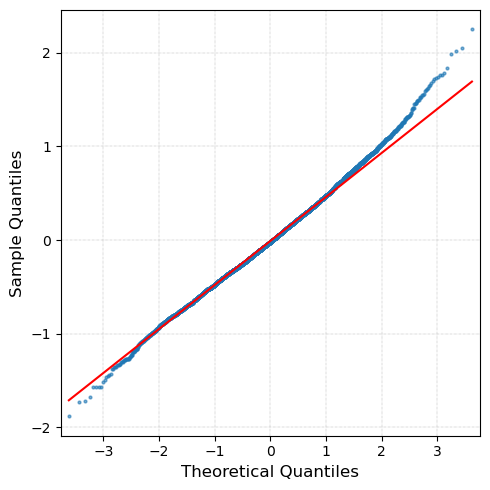
\includegraphics[width=1\linewidth]{ucl-latex-thesis-templates-master/Image/resi_OLS_1.2.png}
  \caption{Q-Q plot.}
  \label{fig:A4.62}
\end{subfigure}
\caption{OLS residuals analysis.}
\label{fig:A4.6}
\end{figure}

%%%%%%%
%%%%%%% Moran I test, LM Robust LM test
%%%%%%%
\begin{table}[]
\centering
\begin{tabular}{|l|l|l|}
\hline
\textbf{Data} & \textbf{Moran I statistic} & \textbf{P-value}  \\ \hline
DMprev        & 0.7931186                  & \textless 2.2e-16 \\ \hline
OLS Residuals & 0.5726112                  & \textless 2.2e-16 \\ \hline
\end{tabular}
\caption{
Moran I test for dependent variable and residuals of OLS model.
}
\label{tab: A4.3}
\end{table}


\begin{table}[]
\centering
\begin{tabular}{|l|l|l|l|}
\hline
\textbf{LM diagnostics} & \textbf{Statistic} & \textbf{P-value} & \textbf{Significance} \\ \hline
LM Lag                  & 4656.03            & \textless 2.2e-16 & ***                   \\ \hline
LM Error                & 5843.65            & \textless 2.2e-16 & ***                   \\ \hline
Robust LM Lag           & 487.13             & \textless 2.2e-16 & ***                   \\ \hline
Robust LM Error         & 1674.75            & \textless 2.2e-16 & ***                   \\ \hline \hline
\multicolumn{4}{|l|}{\textbf{Significance codes:} 0 ‘***’ 0.001 ‘**’ 0.01 ‘*’ 0.05 ‘.’ 0.1 ‘ ’ 1} \\ \hline
\end{tabular}
\caption{
LM diagnostics for spatial dependence
}
\label{tab: A4.4}
\end{table}


\section{Spatial Regression Analysis}
\label{chap:4.4}
Table \ref{tab: A4.5} presents the results of the SLM. We find that the value of Rho is 0.659, indicating a strong spatial dependence in DM prevalence. This means that when DM prevalence in neighboring areas increases by one standard deviation, the DM prevalence in the current area will increase by 0.659 standard deviations. Using Monte Carlo simulations, we calculated the direct effect, indirect effect, and total effect for each variable (see Table \ref{tab: A4.6}). The top three factors with the strongest total effect remain the Asian population, obesity prevalence, and IMD decile. Table \ref{tab: A4.7} presents the results of the SEM. We observe that the lambda value is as high as 0.899, suggesting a strong spatial autocorrelation in the error terms. This indicates that we may have omitted some spatial factors, resulting in spatial dependence that cannot be fully captured by the current independent variables.
Table \ref{tab: A4.8} shows the results of the SDM. Since the SDM is more complex than the SLM, and the regression coefficients for the independent variables cannot be directly compared or interpreted, it is essential to calculate the direct, indirect, and total effects for each variable. Based on Table \ref{tab: A4.9}, using the Asian variable as an example, when the Asian population in the current area increases by one standard deviation compared to the White population, the DM prevalence in the current area will increase by 0.294 standard deviations. When the Asian population in neighboring areas increases by one standard deviation compared to the White population, the DM prevalence in the current area will increase by 0.584 standard deviations. We can see that the top three factors in terms of total effect have shifted to the Asian population, IMD decile, and Age 80+. Obesity prevalence has fallen out of the top three because its indirect effect is not significant, meaning that obesity prevalence in neighboring areas does not have a significant impact on DM prevalence in the current area. We find that the Asian population, IMD decile, and advancing age exhibit strong spatial spillover effects, with their indirect effects exceeding their direct effects.

%%%%%%%
%%%%%%% SLM Table
%%%%%%%
\begin{table}[]
\centering
\begin{tabular}{|lllll|}
\hline
\multicolumn{1}{|l|}{\textbf{Variable}} & \multicolumn{1}{l|}{\textbf{Coefficient}} & \multicolumn{1}{l|}{\textbf{Std. Error}} & \multicolumn{1}{l|}{\textbf{P-value}}  & \textbf{Significance} \\ \hline
\multicolumn{1}{|l|}{(Intercept)}       & \multicolumn{1}{l|}{0.0172885}            & \multicolumn{1}{l|}{0.0039840}           & \multicolumn{1}{l|}{1.428e-05}         & ***                   \\ \hline
\multicolumn{1}{|l|}{Asian}             & \multicolumn{1}{l|}{0.2310246}            & \multicolumn{1}{l|}{0.0062791}           & \multicolumn{1}{l|}{\textless 2.2e-16} & ***                   \\ \hline
\multicolumn{1}{|l|}{Black}             & \multicolumn{1}{l|}{0.0471533}            & \multicolumn{1}{l|}{0.0058128}           & \multicolumn{1}{l|}{4.441e-16}         & ***                   \\ \hline
\multicolumn{1}{|l|}{Mixed}             & \multicolumn{1}{l|}{-0.0640843}           & \multicolumn{1}{l|}{0.0074030}           & \multicolumn{1}{l|}{\textless 2.2e-16} & ***                   \\ \hline
\multicolumn{1}{|l|}{Female}            & \multicolumn{1}{l|}{0.0268484}            & \multicolumn{1}{l|}{0.0043926}           & \multicolumn{1}{l|}{9.829e-10}         & ***                   \\ \hline
\multicolumn{1}{|l|}{Popudensity}       & \multicolumn{1}{l|}{-0.0436492}           & \multicolumn{1}{l|}{0.0059291}           & \multicolumn{1}{l|}{1.814e-13}         & ***                   \\ \hline
\multicolumn{1}{|l|}{Age40\_49}         & \multicolumn{1}{l|}{0.0662121}            & \multicolumn{1}{l|}{0.0056748}           & \multicolumn{1}{l|}{\textless 2.2e-16} & ***                   \\ \hline
\multicolumn{1}{|l|}{Age50\_59}         & \multicolumn{1}{l|}{0.0658630}            & \multicolumn{1}{l|}{0.0062171}           & \multicolumn{1}{l|}{\textless 2.2e-16} & ***                   \\ \hline
\multicolumn{1}{|l|}{Age80}             & \multicolumn{1}{l|}{0.1277811}            & \multicolumn{1}{l|}{0.0063836}           & \multicolumn{1}{l|}{\textless 2.2e-16} & ***                   \\ \hline
\multicolumn{1}{|l|}{OBprev}            & \multicolumn{1}{l|}{0.2281244}            & \multicolumn{1}{l|}{0.0070629}           & \multicolumn{1}{l|}{\textless 2.2e-16} & ***                   \\ \hline
\multicolumn{1}{|l|}{IMDdecile}         & \multicolumn{1}{l|}{-0.2179904}           & \multicolumn{1}{l|}{0.0063877}           & \multicolumn{1}{l|}{\textless 2.2e-16} & ***                   \\ \hline \hline
\multicolumn{1}{|l|}{\textbf{Rho}}               & \multicolumn{1}{l|}{0.65885}              & \multicolumn{1}{l|}{0.0073056}           & \multicolumn{1}{l|}{\textless 2.2e-16} & ***                   \\ \hline \hline
\multicolumn{5}{|l|}{\textbf{Wald statistic:} 8133.1, p-value: \textless 2.22e-16}                                                                                                                       \\ \hline
\multicolumn{5}{|l|}{\textbf{LR test value:} 4741.1, p-value: \textless 2.22e-16}                                                                                                                        \\ \hline
\multicolumn{5}{|l|}{\textbf{Log likelihood:} -2402.065}                                                                                                                                                 \\ \hline
\multicolumn{5}{|l|}{\textbf{AIC:} 4830.13}                                                                                                                                                              \\ \hline
\multicolumn{5}{|l|}{\textbf{BIC:} 4918.834}                                                                                                                                                             \\ \hline \hline
\multicolumn{5}{|l|}{\textbf{Significance codes:} 0 ‘***’ 0.001 ‘**’ 0.01 ‘*’ 0.05 ‘.’ 0.1 ‘ ’ 1}                                                                                                        \\ \hline
\end{tabular}
\caption{
The summary statistics of the SLM.
}
\label{tab: A4.5}
\end{table}


%%%%%%% SLM Impact
\begin{table}[]
\centering
\begin{tabular}{|l||l|l||l|l||l|l|}
\hline
\textbf{Variable} & \multicolumn{2}{c||}{\textbf{Direct}} & \multicolumn{2}{c||}{\textbf{Indirect}} & \multicolumn{2}{c|}{\textbf{Total}} \\ \hline
                  & \textbf{Value} & \textbf{p-value} & \textbf{Value} & \textbf{p-value} & \textbf{Value} & \textbf{p-value} \\ \hline
Asian             & 0.259 & \textless 2.22e-16 & 0.418 & \textless 2.22e-16 & 0.677 & \textless 2.22e-16 \\ \hline
Black             & 0.053 & 2.220e-16 & 0.085 & 2.220e-16 & 0.138 & 2.220e-16 \\ \hline
Mixed             & -0.072 & \textless 2.22e-16 & -0.116 & \textless 2.22e-16 & -0.188 & \textless 2.22e-16 \\ \hline
Female            & 0.030 & 1.346e-09 & 0.049 & 2.047e-09 & 0.079 & 1.510e-09 \\ \hline
Popudensity       & -0.049 & 3.175e-13 & -0.079 & 3.824e-13 & -0.128 & 2.645e-13 \\ \hline
Age40\_49         & 0.074 & \textless 2.22e-16 & 0.120 & \textless 2.22e-16 & 0.194 & \textless 2.22e-16 \\ \hline
Age50\_59         & 0.074 & \textless 2.22e-16 & 0.119 & \textless 2.22e-16 & 0.193 & \textless 2.22e-16 \\ \hline
Age80             & 0.143 & \textless 2.22e-16 & 0.231 & \textless 2.22e-16 & 0.375 & \textless 2.22e-16 \\ \hline
OBprev            & 0.256 & \textless 2.22e-16 & 0.413 & \textless 2.22e-16 & 0.669 & \textless 2.22e-16 \\ \hline
IMDdecile         & -0.245 & \textless 2.22e-16 & -0.394 & \textless 2.22e-16 & -0.639 & \textless 2.22e-16 \\ \hline
\end{tabular}
\caption{
Impact measures and simulated p-values for spatial lag model
}
\label{tab: A4.6}
\end{table}


%%%%%%%
%%%%%%% SEM Table
%%%%%%%
\begin{table}[]
\centering
\begin{tabular}{|lllll|}
\hline
\multicolumn{1}{|l|}{\textbf{Variable}} & \multicolumn{1}{l|}{\textbf{Coefficient}} & \multicolumn{1}{l|}{\textbf{Std. Error}} & \multicolumn{1}{l|}{\textbf{P-value}}  & \textbf{Significance} \\ \hline
\multicolumn{1}{|l|}{(Intercept)}       & \multicolumn{1}{l|}{0.0744906}            & \multicolumn{1}{l|}{0.0334254}           & \multicolumn{1}{l|}{0.0258431}         & *                     \\ \hline
\multicolumn{1}{|l|}{Asian}             & \multicolumn{1}{l|}{0.2810473}            & \multicolumn{1}{l|}{0.0086039}           & \multicolumn{1}{l|}{\textless 2.2e-16} & ***                   \\ \hline
\multicolumn{1}{|l|}{Black}             & \multicolumn{1}{l|}{0.1046913}            & \multicolumn{1}{l|}{0.0088935}           & \multicolumn{1}{l|}{\textless 2.2e-16} & ***                   \\ \hline
\multicolumn{1}{|l|}{Mixed}             & \multicolumn{1}{l|}{-0.1326065}           & \multicolumn{1}{l|}{0.0106191}           & \multicolumn{1}{l|}{\textless 2.2e-16} & ***                   \\ \hline
\multicolumn{1}{|l|}{Female}            & \multicolumn{1}{l|}{0.0154181}            & \multicolumn{1}{l|}{0.0039673}           & \multicolumn{1}{l|}{0.0001018}         & ***                   \\ \hline
\multicolumn{1}{|l|}{Popudensity}       & \multicolumn{1}{l|}{0.0209477}            & \multicolumn{1}{l|}{0.0072549}           & \multicolumn{1}{l|}{0.0038843}         & **                    \\ \hline
\multicolumn{1}{|l|}{Age40\_49}         & \multicolumn{1}{l|}{0.0554306}            & \multicolumn{1}{l|}{0.0060371}           & \multicolumn{1}{l|}{\textless 2.2e-16} & ***                   \\ \hline
\multicolumn{1}{|l|}{Age50\_59}         & \multicolumn{1}{l|}{0.0535536}            & \multicolumn{1}{l|}{0.0058865}           & \multicolumn{1}{l|}{\textless 2.2e-16} & ***                   \\ \hline
\multicolumn{1}{|l|}{Age80}             & \multicolumn{1}{l|}{0.1033838}            & \multicolumn{1}{l|}{0.0058598}           & \multicolumn{1}{l|}{\textless 2.2e-16} & ***                   \\ \hline
\multicolumn{1}{|l|}{OBprev}            & \multicolumn{1}{l|}{0.4645399}            & \multicolumn{1}{l|}{0.0088284}           & \multicolumn{1}{l|}{\textless 2.2e-16} & ***                   \\ \hline
\multicolumn{1}{|l|}{IMDdecile}         & \multicolumn{1}{l|}{-0.2295011}           & \multicolumn{1}{l|}{0.0064026}           & \multicolumn{1}{l|}{\textless 2.2e-16} & ***                   \\ \hline \hline
\multicolumn{1}{|l|}{\textbf{Lambda}}            & \multicolumn{1}{l|}{0.8988}              & \multicolumn{1}{l|}{0.0054564}           & \multicolumn{1}{l|}{\textless 2.2e-16} & ***                   \\ \hline \hline
\multicolumn{5}{|l|}{\textbf{Wald statistic:} 27134, p-value: \textless 2.22e-16}                                                                                                                        \\ \hline
\multicolumn{5}{|l|}{\textbf{LR test value:} 6064, p-value: \textless 2.22e-16}                                                                                                                     \\ \hline
\multicolumn{5}{|l|}{\textbf{Log likelihood:} -1740.616}                                                                                                                                              \\ \hline
\multicolumn{5}{|l|}{\textbf{AIC:} 3507.232}                                                                                                                                                             \\ \hline
\multicolumn{5}{|l|}{\textbf{BIC:} 3595.936}                                                                                                                                                           \\ \hline \hline
\multicolumn{5}{|l|}{\textbf{Significance codes:} 0 ‘***’ 0.001 ‘**’ 0.01 ‘*’ 0.05 ‘.’ 0.1 ‘ ’ 1}                                                                                                      \\ \hline
\end{tabular}
\caption{
The summary statistics of the SEM.
}
\label{tab: A4.7}
\end{table}

%%%%%%%
%%%%%%% SDM Table
%%%%%%%
\begin{table}[]
\centering
\begin{tabular}{|l|l|l|l|l|}
\hline
\textbf{Variable} & \textbf{Coefficient} & \textbf{Std. Error} & \textbf{P-value} & \textbf{Significance} \\ \hline
(Intercept)       & 0.0035706            & 0.0034390           & 0.2991453        &                       \\ \hline
Asian             & 0.2593663            & 0.0090437           & \textless 2.2e-16 & ***                   \\ \hline
Black             & 0.1099056            & 0.0091326           & \textless 2.2e-16 & ***                   \\ \hline
Mixed             & -0.1166722           & 0.0107779           & \textless 2.2e-16 & ***                   \\ \hline
Female            & 0.0152904            & 0.0040001           & 0.0001321        & ***                   \\ \hline
Popudensity       & 0.0322634            & 0.0073054           & 1.004e-05        & ***                   \\ \hline
Age40\_49         & 0.0529707            & 0.0060282           & \textless 2.2e-16 & ***                   \\ \hline
Age50\_59         & 0.0580807            & 0.0059257           & \textless 2.2e-16 & ***                   \\ \hline
Age80             & 0.1071359            & 0.0058703           & \textless 2.2e-16 & ***                   \\ \hline
OBprev            & 0.4453933            & 0.0091057           & \textless 2.2e-16 & ***                   \\ \hline
IMDdecile         & -0.2324876           & 0.0063867           & \textless 2.2e-16 & ***                   \\ \hline \hline
\multicolumn{1}{|l|}{\textbf{Lagged Variable}} & \multicolumn{1}{l|}{\textbf{Coefficient}} & \multicolumn{1}{l|}{\textbf{Std. Error}} & \multicolumn{1}{l|}{\textbf{P-value}}  & \textbf{Significance} \\ \hline
lag.Asian         & -0.1125014           & 0.0121396           & \textless 2.2e-16 & ***                   \\ \hline
lag.Black         & -0.0810433           & 0.0113147           & 7.911e-13        & ***                   \\ \hline
lag.Mixed         & 0.0792986            & 0.0132281           & 2.038e-09        & ***                   \\ \hline
lag.Female        & -0.0021617           & 0.0071244           & 0.7615671        &                       \\ \hline
lag.Popudensity   & -0.0753573           & 0.0099948           & 4.707e-14        & ***                   \\ \hline
lag.Age40\_49     & -0.0372915           & 0.0092084           & 5.128e-05        & ***                   \\ \hline
lag.Age50\_59     & 0.0042647            & 0.0096405           & 0.6582224        &                       \\ \hline
lag.Age80         & -0.0302246           & 0.0106338           & 0.0044788        & **                    \\ \hline
lag.OBprev        & -0.3764927           & 0.0120199           & \textless 2.2e-16 & ***                   \\ \hline
lag.IMDdecile     & 0.1276194            & 0.0104037           & \textless 2.2e-16 & ***                   \\ \hline \hline
\textbf{Rho}              & 0.83342             & 0.0071322           & \textless 2.2e-16 & ***          \\ \hline \hline
\multicolumn{5}{|l|}{\textbf{Wald statistic:} 13655, p-value: \textless 2.22e-16} \\ \hline
\multicolumn{5}{|l|}{\textbf{LR test value:} 5487.5, p-value: \textless 2.22e-16} \\ \hline
\multicolumn{5}{|l|}{\textbf{Log likelihood:} -1508.157} \\ \hline
\multicolumn{5}{|l|}{\textbf{AIC:} 3062.313} \\ \hline
\multicolumn{5}{|l|}{\textbf{BIC:} 3219.25} \\ \hline \hline
\multicolumn{5}{|l|}{\textbf{Significance codes:} 0 ‘***’ 0.001 ‘**’ 0.01 ‘*’ 0.05 ‘.’ 0.1 ‘ ’ 1} \\ \hline
\end{tabular}
\caption{
The summary statistics of the SDM.
}
\label{tab: A4.8}
\end{table}

%%%%%%% SDM Impact
\begin{table}[]
\centering
\begin{tabular}{|l||l|l||l|l||l|l|}
\hline
\textbf{Variable} & \multicolumn{2}{c||}{\textbf{Direct}} & \multicolumn{2}{c||}{\textbf{Indirect}} & \multicolumn{2}{c|}{\textbf{Total}} \\ \hline
                  & \textbf{Value} & \textbf{p-value} & \textbf{Value} & \textbf{p-value} & \textbf{Value} & \textbf{p-value} \\ \hline
Asian             & 0.294 & \textless 2.22e-16 & 0.584 & \textless 2.22e-16 & 0.877 & \textless 2.22e-16 \\ \hline
Black             & 0.114 & \textless 2.22e-16 & 0.059 & 0.111543 & 0.173 & 4.6444e-06 \\ \hline
Mixed             & -0.123 & \textless 2.22e-16 & -0.101 & 0.034351 & -0.223 & 8.3267e-06 \\ \hline
Female            & 0.019 & 9.2171e-05 & 0.060 & 0.109482 & 0.078 & 0.052492 \\ \hline
Popudensity       & 0.016 & 0.037328 & -0.273 & 1.2919e-11 & -0.257 & 1.5203e-09 \\ \hline
Age40\_49         & 0.055 & \textless 2.22e-16 & 0.038 & 0.358950 & 0.093 & 0.037407 \\ \hline
Age50\_59         & 0.076 & \textless 2.22e-16 & 0.297 & 1.4185e-09 & 0.373 & 1.2721e-12 \\ \hline
Age80             & 0.127 & \textless 2.22e-16 & 0.333 & 8.1217e-10 & 0.460 & 2.2204e-15 \\ \hline
OBprev            & 0.444 & \textless 2.22e-16 & -0.032 & 0.382130 & 0.412 & \textless 2.22e-16 \\ \hline
IMDdecile         & -0.255 & \textless 2.22e-16 & -0.372 & 1.3323e-14 & -0.627 & \textless 2.22e-16 \\ \hline
\end{tabular}
\caption{
Impact measures and simulated p-values for SDM
}
\label{tab: A4.9}
\end{table}

\clearpage
\section{Model Selection and Comparison}
\label{chap:4.5}

Table \ref{tab: A4.10} presents the results of the LR test comparing the SDM with the SLM and SEM. We found that both sets of test statistics are very large, and the p-values are significant, indicating that the SDM cannot be simplified to either the SLM or SEM. Additionally, the AIC values for the SLM, SEM, and SDM are 4830.13, 3507.232, and 3062.313, respectively. Their BIC values are 4918.834, 3595.936, and 3219.25, respectively. Therefore, both the AIC and BIC show that the SDM has the lowest values, suggesting that it provides the best fit.
Figure \ref{fig:A4.7} shows the residuals maps of the four regression models we tested. It is clear that the residuals from the OLS model exhibit significant spatial autocorrelation, with most areas of underestimation showing spatial clustering. The SLM reduces some of the spatial autocorrelation, but Moran's I remains significant. The SEM and SDM successfully capture and address the spatial autocorrelation in the data, with Moran's I statistics of 0.01 (p-value greater than 0.05). Given that the SDM provides the best fit and successfully eliminates the spatial autocorrelation in the residuals, and considering Turi's (2017) discussion on spatial spillover effects, the SDM is compelling. Therefore, we have chosen the SDM as our final model.






%%%%%%% SDM LM test for degradation
\begin{table}[]
\centering
\begin{tabular}{|l|l|l|l|}
\hline
\textbf{LR test} & \textbf{Statistic} & \textbf{P-value} & \textbf{Significance} \\ \hline
SDM SLM                  & 1787.82            & \textless 2.2e-16 & ***                   \\ \hline
SDM SEM                & 464.92            & \textless 2.2e-16 & ***                   \\ \hline \hline
\multicolumn{4}{|l|}{\textbf{Significance codes:} 0 ‘***’ 0.001 ‘**’ 0.01 ‘*’ 0.05 ‘.’ 0.1 ‘ ’ 1} \\ \hline
\end{tabular}
\caption{
SDM LR test for degradation
}
\label{tab: A4.10}
\end{table}



\clearpage
\begin{figure}[ht]
\centering
\begin{subfigure}{.4\textwidth}
  \centering
  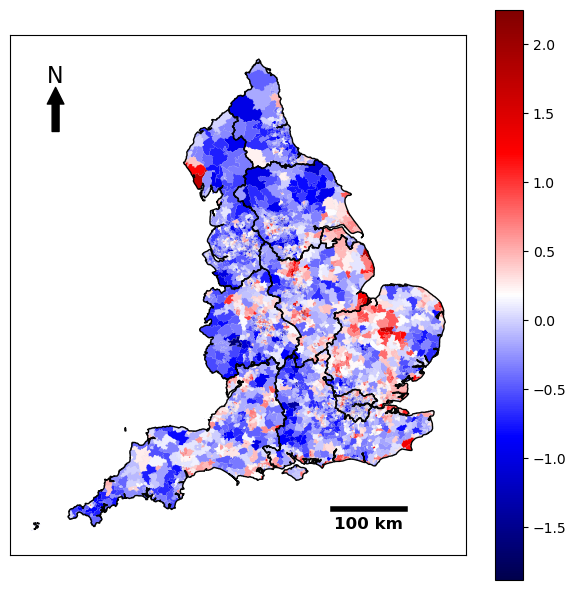
\includegraphics[width=1\linewidth]{ucl-latex-thesis-templates-master/Image/resi_OLS_1.png}
  \caption{OLS.}
  \label{fig:A4.71}
\end{subfigure}%
\begin{subfigure}{.4\textwidth}
  \centering
  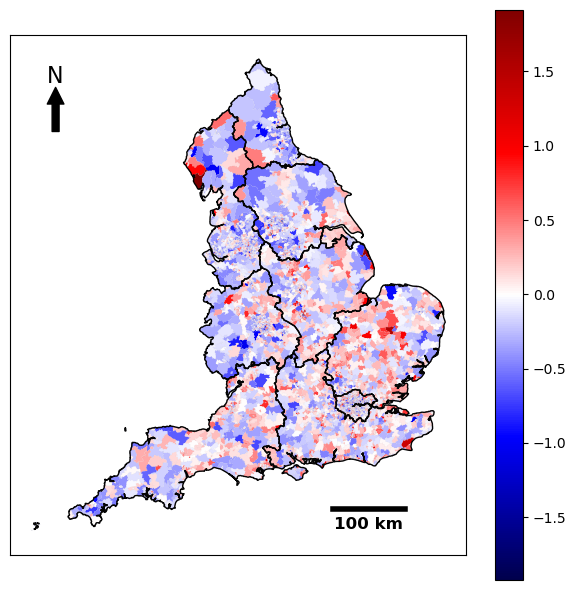
\includegraphics[width=1\linewidth]{ucl-latex-thesis-templates-master/Image/resi_SLM_2.png}
  \caption{SLM.}
  \label{fig:A4.72}
\end{subfigure}
\begin{subfigure}{.4\textwidth}
  \centering
  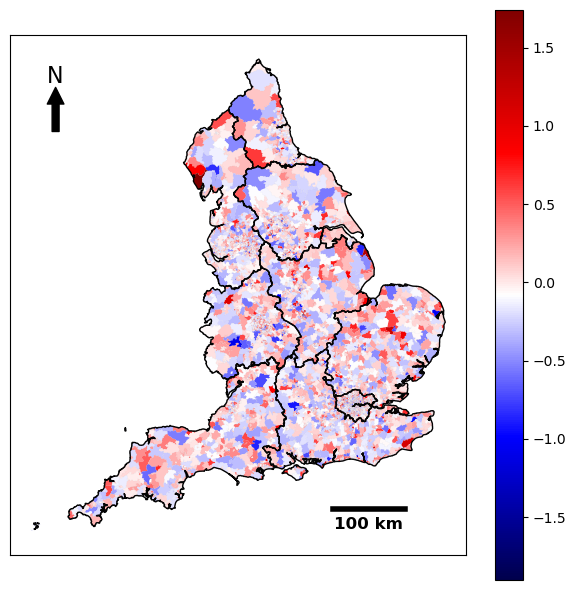
\includegraphics[width=1\linewidth]{ucl-latex-thesis-templates-master/Image/resi_SEM_3.png}
  \caption{SEM.}
  \label{fig:A4.73}
\end{subfigure}
\begin{subfigure}{.4\textwidth}
  \centering
  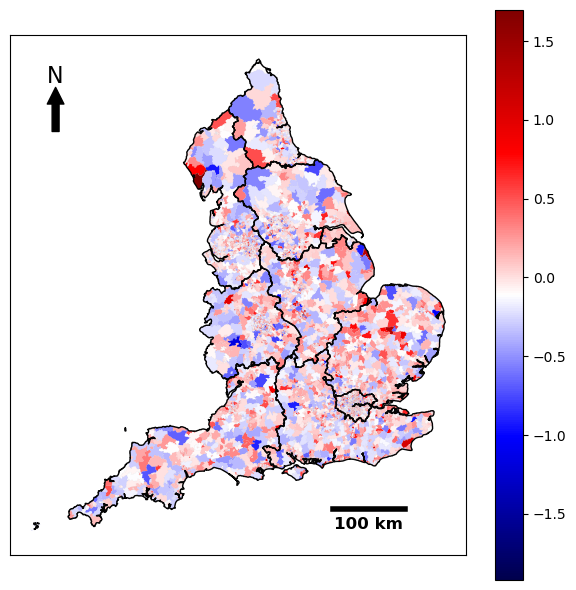
\includegraphics[width=1\linewidth]{ucl-latex-thesis-templates-master/Image/resi_SDM_4.png}
  \caption{SDM.}
  \label{fig:A4.74}
\end{subfigure}
\caption{Residual Maps for each regression model.}
\label{fig:A4.7}
\end{figure}
\chapter{Discussion}
\label{chap:5}

\section{General Discussion}
\label{chap:5.1}
Through initial OLS regression analysis, we found that the Asian population proportion, social deprivation (IMD decile) and obesity prevalence significantly influenced diabetes prevalence. However, significant spatial autocorrelation in the OLS model residuals indicated potential spatial dependency among variables. Thus, we ultimately chose the SDM to better explain these spatial effects.

The SDM results showed that certain variables not only directly impacted diabetes prevalence but also exhibited spatial spillover effects, particularly the Asian population, elderly population proportion and social deprivation. This suggests that population structure and socioeconomic conditions in neighboring areas may significantly affect diabetes prevalence in the current area. Specifically, the research found that when neighboring areas had a higher Asian population proportion, the diabetes prevalence in the current area also increased correspondingly. The elderly population also demonstrated this spatial effect. This may reflect that the area clustering effect of lifestyle, community characteristics and cultural habits of related groups on health status. In England, Asian communities typically have strong cohesion and are concentrated in some large cities. Asian restaurants tend to open in these cohesive communities, further attracting more Asian populations to settle. These restaurants are often concentrated in large cities or around universities, reinforcing the clustering effect of Asian populations in these areas. Moreover, traditional Asian dietary habits are typically rich in carbohydrates, such as rice and noodles. The provision of this diet by restaurants not only meets cultural demands but also, to some extent, promotes the continuation of these dietary habits, potentially increasing the risk of diabetes.

In contrast, whilst the Black population was also significant, it did not exhibit apparent spatial spillover effects, suggesting that the distribution of this group may have a more localized impact on diabetes prevalence without forming widespread spatial effects. Although obesity prevalence showed significant direct effects in the model, it did not demonstrate spatial spillover effects. This implies that the impact of obesity on diabetes prevalence is more confined to specific areas rather than through effects transmitted across neighboring areas. Furthermore, the spillover effect of social deprivation level suggests that economically disadvantaged areas not only have higher diabetes prevalence themselves but their deprived conditions also affect surrounding areas, exacerbating health inequalities in diabetes across different regions. The spillover effect of socioeconomic factors also appeared in Turi's study on DM in the United States (2017), indicating that socioeconomic inequality is an important determinant in many study areas.

The spatial spillover effect of IMD decile suggests that reducing social deprivation is also crucial for diabetes control. Policymakers should strive to reduce socioeconomic inequalities by improving education and employment opportunities, as well as housing and healthcare resources, to lower the risk of diabetes. These measures can not only directly aid deprived areas but also help alleviate pressure on neighboring areas. Regarding obesity, although it did not show apparent spatial spillover effects, its impact in local areas cannot be ignored. Public health strategies should focus on improving people's healthy dietary habits to reduce its direct impact on diabetes. To mitigate the impact of population spillover effects on diabetes prevalence, I suggest promoting health education and preventive measures through institutions such as universities and companies. Universities and companies possess extensive social networks and influence, enabling effective dissemination of knowledge about healthy lifestyles, especially in areas with concentrated high-risk groups.


\section{Limitations}
\label{chap:5.2}
This study also has several limitations. Firstly, there is inconsistency in the temporal alignment of the datasets. For instance, whilst we analyzed diabetes prevalence for 2022/23, the adult dietary data used as an independent variable was modeled based on survey results from 2008-2016 (Smith et al., 2021), potentially raising issues of data obsolescence. Moreover, although we used the 2019 IMD index, which is relatively close to 2022, some of the underlying indicators for IMD were collected at inconsistent and sometimes distant time points. For example, the income indicator is based on 2015 data, which may impact the analysis.
Secondly, although we treated IMD decile as a continuous variable based on literature, to further verify the robustness of results, sensitivity analysis could be conducted, such as coding IMD decile as dummy variables for comparative experiments (Lang et al., 2016).
Thirdly, Soljak et al. (2011) noted that whilst QOF data accurately reflect the prevalence of diagnosed diseases, undiagnosed cases remain a consideration. Future research could incorporate more comprehensive disease prevalence models, such as those provided by the Association of Public Health Observatories, to compare and validate QOF register data, thereby improving the accuracy of diabetes prevalence estimates.
Furthermore, as this study uses ecological data, results cannot be directly applied to individual-level interpretations. This may lead to ecological fallacy, where group-level associations are misinterpreted as individual-level causal relationships, resulting in erroneous inferences (Robinson, 1950). A more reasonable approach would be to use case-control or cohort studies for verification (Elliott and Wartenberg, 2004).
Lastly, cross-sectional studies have limitations in exploring causal relationships. Future research could develop spatiotemporal models to capture more refined spatial distribution and change processes of diabetes, thereby gaining a deeper understanding of the causal relationships between influencing factors and diabetes.
\chapter{Conclusion}
\label{chap:6}

This study identified the significant spatial autocorrelation in DM prevalence in England, indicating a spatial clustering phenomenon in certain areas. Further spatial regression analyses addressed the core research questions and identified several key influencing factors, including Asian population proportions, social deprivation (IMD), and advancing age. Notably, the significant spatial spillover effects of social deprivation and the Asian population suggest that their influence extends beyond specific areas and impacts the surrounding areas through spatial interaction effects. These findings offer an area perspective for future DM prevention and control policies, highlighting the importance of considering not only areas with high prevalence but also the influence of neighboring areas.

The study also found that, although the obesity prevalence was a significant factor in the OLS model, it did not show a spatial spillover effect in the SDM. This may indicate that the effects of obesity are more confined to the individual level rather than spreading through social interactions or neighborhood influences. As a result, future policy interventions may need to prioritize community-level impacts, such as promoting health awareness and healthy lifestyles through public health programs.
Moreover, this study adds a new case to existing spatial epidemiological research, especially in the analysis of noncommunicable diseases. There is considerable potential for further exploration in this area. Future studies could expand the scope of analysis to smaller areas or introduce more complex spatiotemporal dynamic models to track changes in DM prevalence over time.

Despite the valuable insights provided by this study, there are several limitations. First, the ecological nature of the data means that the findings cannot be directly applied to individual-level interpretations. Second, while this study includes a range of socioeconomic and behavioral factors, there may be other potential influences that were not captured. Additionally, while the SDM can reveal spatial spillover effects, cross-sectional studies are limited in their ability to explore causality. Future research could develop spatiotemporal models to capture more detailed spatial distributions and changes in DM prevalence, and better understand the causal relationships between risk factors and DM.

\phantomsection
\addcontentsline{toc}{chapter}{Reference}

\begin{Reference}
%%Introduction reference (14+7 21 reference)
%%LR Section2.1 (19 reference)
%%LR Section2.2 (14 reference)
%%LR Section2.3 (13 reference) 目前总共67个
%%LR Section2.4 ()
%%LR Section2.5 ()
\begin{flushleft}
Alam, U., Asghar, O., Azmi, S., and Malik, R. A. (2014). `General aspects of diabetes mellitus'. \textit{Handbook of clinical neurology}, 126, pp.211-222.
\end{flushleft}
\vspace{2pt}


\begin{flushleft}
Albert, D. P., Gesler, W. M., and Levergood, B. (eds.) (2000). \textit{Spatial analysis, GIS, and remote sensing applications in the health sciences}. Chelsea, MI: Ann Arbor Press.
\end{flushleft}
\vspace{2pt}


\begin{flushleft}
Anselin, L. (2005). `Exploring spatial data with GeoDaTM: a workbook'. \textit{Centre for Spatially Integrated Social Science}.
\end{flushleft}
\vspace{2pt}


\begin{flushleft}
Anselin, L., and Bera, A. K. (1998). `Spatial dependence in linear regression models with an introduction to spatial econometrics'. \textit{Statistics textbooks and monographs}, 155, pp.237-290.
\end{flushleft}
\vspace{2pt}


\begin{flushleft}
Artiga, S., and Hinton, E. (2018). `Beyond health care: the role of social determinants in promoting health and health equity'. \textit{Kaiser Family Foundation}, 10.
\end{flushleft}
\vspace{2pt}


\begin{flushleft}
Askari, M. H., Gupta, K., and Bengal, W. (2016). `Conceptualising medical geography'. \textit{Transactions}, 38(1), p.127.
\end{flushleft}
\vspace{2pt}


\begin{flushleft}
Baker, C. (2024). \textit{Constituency data: health conditions}. UK Parliament, House of Commons Library. Available at: \url{https://commonslibrary.parliament.uk/constituency-data-how-healthy-is-your-area/} (Accessed: 21 July 2024).
\end{flushleft}
\vspace{7pt}


\begin{flushleft}
Baker, C. (2021). \textit{Local health conditions prevalence estimates based on QOF}. GitHub repository. Available at: \url{https://github.com/houseofcommonslibrary/local-health-data-from-QOF} (Accessed: 15 July 2024).
\end{flushleft}
\vspace{7pt}


\begin{flushleft}
Berkman, L. F., Kawachi, I., and Glymour, M. M. (eds.) (2014). \textit{Social epidemiology}. Oxford University Press.
\end{flushleft}
\vspace{2pt}


\begin{flushleft}
Bilal, U., Auchincloss, A. H., and Diez-Roux, A. V. (2018). `Neighborhood environments and diabetes risk and control'. \textit{Current diabetes reports}, 18, pp.1-10.
\end{flushleft}
\vspace{2pt}


\begin{flushleft}
Boehme, A. K., Esenwa, C., and Elkind, M. S. (2017). `Stroke risk factors, genetics, and prevention'. \textit{Circulation research}, 120(3), pp.472-495.
\end{flushleft}
\vspace{2pt}


\begin{flushleft}
Borgnakke, W. S. (2016). `Modifiable risk factors for periodontitis and diabetes'. \textit{Current Oral Health Reports}, 3, pp.254-269.
\end{flushleft}
\vspace{2pt}


\begin{flushleft}
Borgnakke, W. S. (2016). `Non-modifiable risk factors for periodontitis and diabetes'. \textit{Current oral health reports}, 3, pp.270-281.
\end{flushleft}
\vspace{2pt}


\begin{flushleft}
Braveman, P. (2014). `What are health disparities and health equity? We need to be clear'. \textit{Public health reports}, 129(1\_suppl2), pp.5-8.
\end{flushleft}
\vspace{2pt}


\begin{flushleft}
Brown, A. F., Ettner, S. L., Piette, J., Weinberger, M., Gregg, E., Shapiro, M. F., Karter, A. J., Safford, M., et al. (2004). `Socioeconomic position and health among persons with diabetes mellitus: a conceptual framework and review of the literature'. \textit{Epidemiologic reviews}, 26(1), pp.63-77.
\end{flushleft}
\vspace{2pt}


\begin{flushleft}
Centers for Disease Control and Prevention (2024). \textit{Diabetes Risk Factors}. Available at: \url{https://www.cdc.gov/diabetes/risk-factors/index.html} (Accessed: 10 July 2024).
\end{flushleft}
\vspace{2pt}


\begin{flushleft}
Cuadros, D. F., Li, J., Musuka, G., and Awad, S. F. (2021). `Spatial epidemiology of diabetes: methods and insights'. \textit{World journal of diabetes}, 12(7), p.1042.
\end{flushleft}
\vspace{2pt}


\begin{flushleft}
Dagogo-Jack, S. (ed.) (2017). \textit{Diabetes mellitus in developing countries and underserved communities}. Springer International Publishing.
\end{flushleft}
\vspace{2pt}


\begin{flushleft}
Daneman, D. (2006). `Type 1 diabetes'. \textit{The Lancet}, 367(9513), pp.847-858.
\end{flushleft}
\vspace{2pt}


\begin{flushleft}
Dankwa-Mullan, I., Rhee, K. B., Williams, K., Sanchez, I., Sy, F. S., Stinson Jr, N., and Ruffin, J. (2010). `The science of eliminating health disparities: summary and analysis of the NIH summit recommendations'. \textit{American journal of public health}, 100(S1), S12-S18.
\end{flushleft}
\vspace{2pt}


\begin{flushleft}
de Wit, M., Trief, P. M., Huber, J. W., and Willaing, I. (2020). `State of the art: understanding and integration of the social context in diabetes care'. \textit{Diabetic Medicine}, 37(3), pp.473-482.
\end{flushleft}
\vspace{2pt}


\begin{flushleft}
Elliott, P., and Wartenberg, D. (2004). `Spatial epidemiology: current approaches and future challenges'. \textit{Environmental health perspectives}, 112(9), pp.998-1006.
\end{flushleft}
\vspace{2pt}


\begin{flushleft}
Epifano, L., Di Vincenzo, A., Fanelli, C., Porcellati, E., Perriello, G., De Feo, P., Motolese, M., Brunetti, P., et al. (1992). `Effect of cigarette smoking and of a transdermal nicotine delivery system on glucoregulation in type 2 diabetes mellitus'. \textit{European journal of clinical pharmacology}, 43, pp.257-263.
\end{flushleft}
\vspace{2pt}


\begin{flushleft}
Ford, E., Boyd, A., Bowles, J. K., Havard, A., Aldridge, R. W., Curcin, V., Greiver, M., Harron, K., et al. (2019). `Our data, our society, our health: A vision for inclusive and transparent health data science in the United Kingdom and beyond'. \textit{Learning health systems}, 3(3), e10191.
\end{flushleft}
\vspace{7pt}


\begin{flushleft}
Frati, A. C., Iniestra, F., and Ariza, C. R. (1996). `Acute effect of cigarette smoking on glucose tolerance and other cardiovascular risk factors'. \textit{Diabetes care}, 19(2), pp.112-118.
\end{flushleft}
\vspace{2pt}


\begin{flushleft}
Gebreab, S. Y., Hickson, D. A., Sims, M., Wyatt, S. B., Davis, S. K., Correa, A., and Diez-Roux, A. V. (2017). `Neighborhood social and physical environments and type 2 diabetes mellitus in African Americans: The Jackson Heart Study'. \textit{Health \& place}, 43, pp.128-137.
\end{flushleft}
\vspace{2pt}


\begin{flushleft}
Goldstein, B. J. (2002). `Insulin resistance as the core defect in type 2 diabetes mellitus'. \textit{The American journal of cardiology}, 90(5), pp.3-10.
\end{flushleft}
\vspace{2pt}


\begin{flushleft}
González, E. M., Johansson, S., Wallander, M. A., and Rodríguez, L. G. (2009). `Trends in the prevalence and incidence of diabetes in the UK: 1996–2005'. \textit{Journal of Epidemiology \& Community Health}, 63(4), pp.332-336.
\end{flushleft}
\vspace{2pt}


\begin{flushleft}
Henning, R. J. (2018). `Type-2 diabetes mellitus and cardiovascular disease'. \textit{Future cardiology}, 14(6), pp.491-509.
\end{flushleft}
\vspace{2pt}


\begin{flushleft}
Hex, N., MacDonald, R., Pocock, J., Uzdzinska, B., Taylor, M., Atkin, M., Wild, S., Beba, H., et al. (2024). `Estimation of the direct health and indirect societal costs of diabetes in the UK using a cost of illness model'. \textit{Diabetic Medicine}, e15326.
\end{flushleft}
\vspace{2pt}


\begin{flushleft}
Hill-Briggs, F., Adler, N. E., Berkowitz, S. A., Chin, M. H., Gary-Webb, T. L., Navas-Acien, A., Thornton, P. L. and Haire-Joshu, D. (2021). `Social determinants of health and diabetes: a scientific review'. \textit{Diabetes care}, 44(1), p.258.
\end{flushleft}
\vspace{2pt}


\begin{flushleft}
InterAct Consortium robert. (2013). `The link between family history and risk of type 2 diabetes is not explained by anthropometric, lifestyle or genetic risk factors: the EPIC-InterAct study', \textit{Diabetologia}, 56, pp.60-69.
\end{flushleft}
\vspace{2pt}


\begin{flushleft}
James, J. (2015). \textit{The health of populations: Beyond medicine}. Academic Press.
\end{flushleft}
\vspace{2pt}


\begin{flushleft}
Jonsson, B. (1998). `The economic impact of diabetes'. \textit{Diabetes care}, 21(Supplement\_3), C7-C10.
\end{flushleft}
\vspace{2pt}


\begin{flushleft}
Klein, S., Gastaldelli, A., Yki-Järvinen, H., and Scherer, P. E. (2022). `Why does obesity cause diabetes?'. \textit{Cell metabolism}, 34(1), pp.11-20.
\end{flushleft}
\vspace{2pt}


\begin{flushleft}
Knott, C., Bell, S., and Britton, A. (2015). `Alcohol consumption and the risk of type 2 diabetes: a systematic review and dose-response meta-analysis of more than 1.9 million individuals from 38 observational studies'. \textit{Diabetes care}, 38(9), pp.1804-1812.
\end{flushleft}
\vspace{2pt}


\begin{flushleft}
Lang, S. J., Abel, G. A., Mant, J., and Mullis, R. (2016). `Impact of socioeconomic deprivation on screening for cardiovascular disease risk in a primary prevention population: a cross-sectional study'. \textit{BMJ open}, 6(3), e009984.
\end{flushleft}
\vspace{2pt}


\begin{flushleft}
Levene, L. S., Baker, R., Bankart, J., Walker, N., and Wilson, A. (2019). `Socioeconomic deprivation scores as predictors of variations in NHS practice payments: a longitudinal study of English general practices 2013–2017'. \textit{British Journal of General Practice}, 69(685), e546-e554.
\end{flushleft}
\vspace{2pt}


\begin{flushleft}
Lewer, D., Aldridge, R. W., Menezes, D., Sawyer, C., Zaninotto, P., Dedicoat, M., Ahmed, I., Luchenski, S., et al. (2019). `Health-related quality of life and prevalence of six chronic diseases in homeless and housed people: a cross-sectional study in London and Birmingham, England'. \textit{BMJ open}, 9(4), e025192.
\end{flushleft}
\vspace{2pt}


\begin{flushleft}
Maier, W. (2017). `Indices of multiple deprivation for the analysis of regional health disparities in Germany: experiences from epidemiology and healthcare research'. \textit{Bundesgesundheitsblatt-Gesundheitsforschung-Gesundheitsschutz}, 60, pp.1403-1412.
\end{flushleft}
\vspace{2pt}


\begin{flushleft}
Malik, V. S., Popkin, B. M., Bray, G. A., Després, J. P., Willett, W. C., and Hu, F. B. (2010). `Sugar-sweetened beverages and risk of metabolic syndrome and type 2 diabetes: a meta-analysis'. \textit{Diabetes care}, 33(11), pp.2477-2483.
\end{flushleft}
\vspace{2pt}


\begin{flushleft}
Marill, T., and Green, D. (1963). `On the effectiveness of receptors in recognition systems'. \textit{IEEE transactions on Information Theory}, 9 (1), pp.11-17.
\end{flushleft}
\vspace{2pt}


\begin{flushleft}
Marks, J. B., and Raskin, P. (2000). `Cardiovascular risk in diabetes: a brief review'. \textit{Journal of Diabetes and its Complications}, 14(2), pp.108-115.
\end{flushleft}
\vspace{2pt}


\begin{flushleft}
Marmot, M., and Allen, J. J. (2014). `Social determinants of health equity'. \textit{American journal of public health}, 104(S4), S517-S519.
\end{flushleft}
\vspace{2pt}


\begin{flushleft}
McLafferty, S. L. (2003). `GIS and health care'. \textit{Annual review of public health}, 24(1), pp.25-42.
\end{flushleft}
\vspace{2pt}


\begin{flushleft}
McLeod, K. S. (2000). `Our sense of Snow: the myth of John Snow in medical geography'. \textit{Social science \& medicine}, 50(7-8), pp.923-935.
\end{flushleft}
\vspace{2pt}


\begin{flushleft}
Ministry of Housing, Communities and Local Government (2019). \textit{English indices of deprivation 2019}. Available at: \url{https://www.gov.uk/government/statistics/english-indices-of-deprivation-2019} (Accessed: 21 May 2024).
\end{flushleft}
\vspace{2pt}


\begin{flushleft}
Ministry of Housing, Communities and Local Government (2019). \textit{The English Indices of Deprivation 2019 Research report}. Available at: \url{https://assets.publishing.service.gov.uk/media/5d8b364ced915d03709e3cf2/IoD2019_Research_Report.pdf} (Accessed: 15 June 2024).
\end{flushleft}
\vspace{2pt}


\begin{flushleft}
Ministry of Housing, Communities and Local Government (2019). \textit{The English Indices of Deprivation 2019 (IoD2019) Statistical Release}. Available at: \url{https://assets.publishing.service.gov.uk/media/5d8e26f6ed915d5570c6cc55/IoD2019_Statistical_Release.pdf} (Accessed: 15 June 2024).
\end{flushleft}
\vspace{2pt}


\begin{flushleft}
Moore, D. A., and Carpenter, T. E. (1999). `Spatial analytical methods and geographic information systems: use in health research and epidemiology'. \textit{Epidemiologic reviews}, 21(2), pp.143-161.
\end{flushleft}
\vspace{2pt}


\begin{flushleft}
Muir, K., Rattanamongkolgul, S., Smallman-Raynor, M., Thomas, M., Downer, S., and Jenkinson, C. (2004). `Breast cancer incidence and its possible spatial association with pesticide application in two counties of England'. \textit{Public health}, 118(7), pp.513-520.
\end{flushleft}
\vspace{2pt}


\begin{flushleft}
Myerson, R., Lu, T., Peters, A., Fox, S., and Huang, E. (2020). `Impact of health insurance policy on diabetes management'. \textit{Behavioral Diabetes: Social Ecological Perspectives for Pediatric and Adult Populations}, pp.491-504.
\end{flushleft}
\vspace{2pt}


\begin{flushleft}
Nazarko, L. (2023). `Type 2 diabetes: An overview of risk factors and prevention of onset'. \textit{Nursing Times}, 2.
\end{flushleft}
\vspace{2pt}


\begin{flushleft}
NHS England (2023). \textit{National Diabetes Audit 2021-22, Report 1: Care Processes and Treatment Targets, Detailed Analysis Report}. Available at: \url{https://digital.nhs.uk/data-and-information/publications/statistical/national-diabetes-audit/report-1-care-processes-and-treatment-targets-2021-22-full-report} (Accessed: 15 June 2024).
\end{flushleft}
\vspace{2pt}


\begin{flushleft}
NHS England (2022). \textit{NHS prevention programme cuts chances of type 2 diabetes for thousands}. Available at: \url{https://www.england.nhs.uk/2022/03/nhs-prevention-programme-cuts-chances-of-type-2-diabetes-for-thousands/} (Accessed: 15 June 2024).
\end{flushleft}
\vspace{2pt}


\begin{flushleft}
NHS England. (2020). \textit{Patients Registered at a GP Practice January 2020; Special Topic}. Available at: \url{https://digital.nhs.uk/data-and-information/publications/statistical/patients-registered-at-a-gp-practice/january-2020} (Accessed: 14 June 2024).
\end{flushleft}
\vspace{7pt}


\begin{flushleft}
NHS England (2024). \textit{Quality and Outcomes Framework}. Available at: \url{https://qof.digital.nhs.uk} (Accessed: 21 July 2024).
\end{flushleft}
\vspace{7pt}


\begin{flushleft}
NHS England (2023). \textit{Quality and Outcomes Framework, 2022-23}. Available at: \url{https://digital.nhs.uk/data-and-information/publications/statistical/quality-and-outcomes-framework-achievement-prevalence-and-exceptions-data/2022-23} (Accessed: 21 July 2024).
\end{flushleft}
\vspace{7pt}


\begin{flushleft}
NHS England (2022). \textit{Update on Quality Outcomes Framework changes for 2022/23}
\url{https://www.england.nhs.uk/wp-content/uploads/2022/03/B1333_Update-on-Quality-Outcomes-Framework-changes-for-2022-23_310322.pdf} (Accessed: 21 July 2024).
\end{flushleft}
\vspace{7pt}


\begin{flushleft}
Nykiforuk, C. I., and Flaman, L. M. (2011). `Geographic information systems (GIS) for health promotion and public health: a review'. \textit{Health promotion practice}, 12(1), pp.63-73.
\end{flushleft}
\vspace{2pt}


\begin{flushleft}
Office for Health Improvement and Disparities (2023). \textit{Child and maternal health statistics}. Available at: \url{https://www.gov.uk/government/collections/child-and-maternal-health-statistics#overview-of-child-health-and-child-health-profiles} (Accessed: 14 July 2024).
\end{flushleft}
\vspace{2pt}


\begin{flushleft}
Office for Health Improvement and Disparities (2017). \textit{Local Alcohol Profiles for England (LAPE)}. Available at: \url{https://www.gov.uk/government/collections/local-alcohol-profiles-for-england-lape} (Accessed: 14 July 2024).
\end{flushleft}
\vspace{2pt}


\begin{flushleft}
Office for Health Improvement and Disparities (no date). \textit{Statistics on OHID}. Available at: \url{https://www.gov.uk/government/organisations/office-for-health-improvement-and-disparities/about/statistics} (Accessed: 20 June 2024).
\end{flushleft}
\vspace{2pt}


\begin{flushleft}
Office for National Statistics. (2021). \textit{Census}. Available at: \url{https://www.ons.gov.uk/census} (Accessed: 1 June 2024).
\end{flushleft}
\vspace{7pt}


\begin{flushleft}
Office for National Statistics. (2024). \textit{Middle layer Super Output Area population estimates}. Available at: \url{https://www.ons.gov.uk/peoplepopulationandcommunity/populationandmigration/populationestimates/datasets/middlesuperoutputareamidyearpopulationestimates} (Accessed: 1 June 2024).
\end{flushleft}
\vspace{7pt}


\begin{flushleft}
Office for National Statistics (2024). \textit{MSOA (2011) to MSOA (2021) to Local Authority District (2022) Exact Fit Lookup for EW (V2)}. Available at: \url{https://www.data.gov.uk/dataset/da36cac8-51c4-4d68-a4a9-37ac47d2a4ba/msoa-2011-to-msoa-2021-to-local-authority-district-2022-exact-fit-lookup-for-ew-v2} (Accessed: 20 June 2024).
\end{flushleft}
\vspace{2pt}


\begin{flushleft}
Office for National Statistics (2021). \textit{Output Area (2011) to LSOA (2011) to MSOA (2011) LAD to LEP (April 2021) Best Fit Lookup in EN (V3)}. Available at: \url{https://geoportal.statistics.gov.uk/documents/698bb0f385914f79bc68298700acdba8/about} (Accessed: 20 June 2024).
\end{flushleft}
\vspace{2pt}


\begin{flushleft}
Office for National Statistics (no date). \textit{Statistical geographies}. Available at: \url{https://www.ons.gov.uk/methodology/geography/ukgeographies/statisticalgeographies} (Accessed: 1 June 2024).
\end{flushleft}
\vspace{2pt}


\begin{flushleft}
Osayomi, T. (2019). `The emergence of a diabetes pocket in Nigeria: The result of a spatial analysis'. \textit{GeoJournal}, 84, pp.1149-1164.
\end{flushleft}
\vspace{2pt}


\begin{flushleft}
Ozougwu, J. C., Obimba, K. C., Belonwu, C. D., and Unakalamba, C. B. (2013). `The pathogenesis and pathophysiology of type 1 and type 2 diabetes mellitus'. \textit{J Physiol Pathophysiol}, 4(4), pp.46-57.
\end{flushleft}
\vspace{2pt}


\begin{flushleft}
Patnaik, C. and Dutta, A. (2023). `Green finance and economic efficiency in India and regional disparity: An inquiry into its influence using spatial data analysis'. \textit{Journal of Advanced Zoology}, 44, pp. 4169-4179.
\end{flushleft}
\vspace{2pt}


\begin{flushleft}
Payne, R. A., and Abel, G. A. (2012). `UK indices of multiple deprivation-a way to make comparisons across constituent countries easier'. \textit{Health Stat Q}, 53(22), pp.2015-2016.
\end{flushleft}
\vspace{2pt}


\begin{flushleft}
Pettitt, D. J., Talton, J., Dabelea, D., Divers, J., Imperatore, G., Lawrence, J. M., Liese, A. D., Linder, B., et al. (2014). `Prevalence of diabetes in US youth in 2009: the SEARCH for diabetes in youth study'. \textit{Diabetes care}, 37(2), pp.402-408.
\end{flushleft}
\vspace{2pt}


\begin{flushleft}
Pham, T. M., Carpenter, J. R., Morris, T. P., Sharma, M., and Petersen, I. (2019). `Ethnic differences in the prevalence of type 2 diabetes diagnoses in the UK: cross-sectional analysis of the health improvement network primary care database'. \textit{Clinical epidemiology}, pp.1081-1088.
\end{flushleft}
\vspace{2pt}


\begin{flushleft}
Public Health England (2014). \textit{Adult obesity and type 2 diabetes}. Available at: \url{https://assets.publishing.service.gov.uk/media/5a7f069140f0b6230268d059/Adult_obesity_and_type_2_diabetes_.pdf} (Accessed: 21 June 2024).
\end{flushleft}
\vspace{2pt}


\begin{flushleft}
Public Health England (2016). \textit{Diabetes prevalence model: Briefing paper}. Available at: \url{https://assets.publishing.service.gov.uk/media/5a82c07340f0b6230269c82d/Diabetesprevalencemodelbriefing.pdf} (Accessed: 21 June 2024).
\end{flushleft}
\vspace{2pt}


\begin{flushleft}
Qi, X., Jia, Y., Pan, C., Li, C., Wen, Y., Hao, J., and Zhang, F. (2022). `Index of multiple deprivation contributed to common psychiatric disorders: a systematic review and comprehensive analysis'. \textit{Neuroscience \& Biobehavioral Reviews}, 140, 104806.
\end{flushleft}
\vspace{2pt}


\begin{flushleft}
Rajpal, A., Rahimi, L., and Ismail‐Beigi, F. (2020). `Factors leading to high morbidity and mortality of COVID‐19 in patients with type 2 diabetes'. \textit{Journal of diabetes}, 12(12), pp.895-908.
\end{flushleft}
\vspace{2pt}


\begin{flushleft}
Ramachandran, A. (2014). `Know the signs and symptoms of diabetes'. \textit{Indian Journal of Medical Research}, 140(5), pp.579-581.
\end{flushleft}
\vspace{2pt}


\begin{flushleft}
Robinson, W. S. (1950). `Ecological correlations and the behavior of individuals'. \textit{International journal of epidemiology}, 38(2), pp.337-341.
\end{flushleft}
\vspace{2pt}


\begin{flushleft}
Rose, G. (2001). `Sick individuals and sick populations'. \textit{International journal of epidemiology}, 30(3), pp.427-432.
\end{flushleft}
\vspace{2pt}


\begin{flushleft}
Shang, M., Zhang, S. and Yang, Q. (2024). `The spatial role and influencing mechanism of the digital economy in empowering high-quality economic development'. \textit{Sustainability}, 16, p. 1425.
\end{flushleft}
\vspace{2pt}


\begin{flushleft}
Smith, D. M., Vogel, C., Campbell, M., Alwan, N. and Moon, G. (2021). `Adult diet in England: Where is more support needed to achieve dietary recommendations?'. \textit{Plos one}, 16(6), e0252877.
\end{flushleft}
\vspace{7pt}


\begin{flushleft}
Solar, O., and Irwin, A. (2010). \textit{A conceptual framework for action on the social determinants of health}. WHO Document Production Services.
\end{flushleft}
\vspace{2pt}


\begin{flushleft}
Soljak, M., Samarasundera, E., Indulkar, T., Walford, H., and Majeed, A. (2011). `Variations in cardiovascular disease under-diagnosis in England: national cross-sectional spatial analysis'. \textit{BMC cardiovascular disorders}, 11, pp.1-11.
\end{flushleft}
\vspace{2pt}


\begin{flushleft}
Strong, M., Maheswaran, R., Pearson, T., and Fryers, P. (2007). `A method for modelling GP practice level deprivation scores using GIS'. \textit{International Journal of Health Geographics}, 6, pp.1-11.
\end{flushleft}
\vspace{2pt}


\begin{flushleft}
Strong, M., Maheswaran, R., and Radford, J. (2006). `Socioeconomic deprivation, coronary heart disease prevalence and quality of care: a practice-level analysis in Rotherham using data from the new UK general practitioner Quality and Outcomes Framework'. \textit{Journal of Public Health}, 28(1), pp.39-42.
\end{flushleft}
\vspace{2pt}


\begin{flushleft}
Sun, Y., Hu, X., Huang, Y., and On Chan, T. (2020). `Spatial patterns of childhood obesity prevalence in relation to socioeconomic factors across England'. \textit{ISPRS International Journal of Geo-Information}, 9(10), p.599.
\end{flushleft}
\vspace{2pt}


\begin{flushleft}
Sun, Y., Hu, X., and Xie, J. (2021). `Spatial inequalities of COVID-19 mortality rate in relation to socioeconomic and environmental factors across England'. \textit{Science of the total environment}, 758, 143595.
\end{flushleft}
\vspace{2pt}


\begin{flushleft}
Tene, O. and Polonetsky, J. (2012). `Big data for all: Privacy and user control in the age of analytics'. \textit{Nw. J. Tech. \& Intell. Prop.}, 11, 239.
\end{flushleft}
\vspace{7pt}


\begin{flushleft}
The Scottish Public Health Observatory (2023). \textit{Risk factors: overview}. Available at: \url{https://www.scotpho.org.uk/risk-factors/} (Accessed: 25 June 2024).
\end{flushleft}
\vspace{2pt}


\begin{flushleft}
Tonstad, S., Butler, T., Yan, R., and Fraser, G. E. (2009). `Type of vegetarian diet, body weight, and prevalence of type 2 diabetes'. \textit{Diabetes care}, 32(5), pp.791-796.
\end{flushleft}
\vspace{2pt}


\begin{flushleft}
Turi, K. N., and Grigsby-Toussaint, D. S. (2017). `Spatial spillover and the socio-ecological determinants of diabetes-related mortality across US counties'. \textit{Applied geography}, 85, pp.62-72.
\end{flushleft}
\vspace{2pt}


\begin{flushleft}
Willi, C., Bodenmann, P., Ghali, W. A., Faris, P. D., and Cornuz, J. (2007). `Active smoking and the risk of type 2 diabetes: a systematic review and meta-analysis'. \textit{Jama}, 298(22), pp.2654-2664.
\end{flushleft}
\vspace{2pt}


\begin{flushleft}
Whitehouse, S. (2018). \textit{Estimating the diagnosis of health conditions}. Available at: \url{http://dataunlocked.co.uk/estimating-the-diagnosis-of-health-conditions/?doing_wp_cron=1719750389.6598451137542724609375} (Accessed: 7 July 2024).
\end{flushleft}
\vspace{2pt}


\begin{flushleft}
WHO Commission on Social Determinants of Health, and World Health Organization. (2008). \textit{Closing the gap in a generation: health equity through action on the social determinants of health: Commission on Social Determinants of Health final report}. World Health Organization.
\end{flushleft}
\vspace{2pt}


\begin{flushleft}
World Health Organization (2023). \textit{Diabetes}. Available at: \url{https://www.who.int/news-room/fact-sheets/detail/diabetes} (Accessed: 14 June 2024).
\end{flushleft}
\vspace{2pt}


\begin{flushleft}
World Health Organization (no date). \textit{Health Inequality Monitor}. Available at: \url{https://www.who.int/data/inequality-monitor} (Accessed: 20 June 2024).
\end{flushleft}
\vspace{2pt}


\begin{flushleft}
World Health Organization (no date). \textit{World Diabetes Day}. Available at: \url{https://www.who.int/campaigns/world-diabetes-day} (Accessed: 14 June 2024).
\end{flushleft}
\vspace{2pt}


\begin{flushleft}
You, H., Zhou, D., Wu, S., Hu, X., and Bie, C. (2020). `Social deprivation and rural public health in China: exploring the relationship using spatial regression'. \textit{Social indicators research}, 147, pp.843-864.
\end{flushleft}
\vspace{2pt}







\end{Reference}













\phantomsection
\addcontentsline{toc}{chapter}{Appendices}

% The \appendix command resets the chapter counter, and changes the chapter numbering scheme to capital letters.
%\chapter{Appendices}
\appendix
\chapter{Research Log}
\label{appendixlabel1}
\begin{table}[H]
\captionsetup{justification=centering}
\centering
\begin{tabular}{|p{3cm}|p{10cm}|}
\hline
\textbf{Timeline} & \textbf{Tasks} \\
\hline \hline
April----May  & This month, in-depth discussions were held, the initial proposal was developed, and the ethics form was submitted. During the first discussion with my supervisor on the 8th of April, I gained an understanding of the ethics form submission process and organised the research questions and framework. \\
\hline \hline
May----June & This month, relevant datasets were identified, and research methods were carefully considered. I also read some related literature. On the 16th of May, I submitted the checklist required by my supervisor. In the meeting with my supervisor on the 17th of May, we discussed the research framework and ideas, and I reviewed the literature. \\
\hline \hline
June----July & This month, I further explored and adjusted the methods. On the 7th of June, I participated in a drop-in discussion, where the supervisor provided substantial help with the methods and tutorial materials. On the 20th of June, I submitted another checklist as required by the supervisor, and on the 21st of June, I participated in the dissertation mini symposium organised by the supervisor. \\
\hline \hline
July----August & This month, I explored the data and drafted the rough code. On the 15th of July, I submitted a draft of the code, considering minor adjustments to the research questions. On the 17th of July, I met with the supervisor to discuss these methodological adjustments. \\
\hline \hline
August----End & The findings were discussed and finalised this month. The code draft was resubmitted on the 9th of August, and I met with the supervisor again on the 12th of August to discuss the findings, including the interpretation of the results and any necessary adjustments. \\
\hline
\end{tabular}
\end{table}





 
% You could separate these out into different files if you have
%  particularly large appendices.

% Actually generates your bibliography. The fact that \include is 
% the last thing before this ensures that it is on a clear page.
%%%\bibliography{example}

% All done. \o/
\end{document}
